\documentclass[a4paper]{report}
\title{PhD Thesis}
\author{Fintan S. Nagle}



%BEGIN MATRIX GUMF
% Load TikZ
\usepackage{tikz}
\usetikzlibrary{matrix,decorations.pathreplacing,calc}

\usepackage[mediumspace,mediumqspace,Grey,squaren]{SIunits}
\usepackage{subfigure}
 \usepackage{graphicx}
 \usepackage{mathtools}
 \usepackage{amsmath}
 \usepackage{setspace}
 \usepackage{tikz}

\newenvironment{enoomerate}{
\begin{enumerate}
  \setlength{\itemsep}{1pt}
  \setlength{\parskip}{0pt}
  \setlength{\parsep}{0pt}}{\end{enumerate}
}

\newenvironment{itemise}{
\begin{itemize}
  \setlength{\itemsep}{1pt}
  \setlength{\parskip}{0pt}
  \setlength{\parsep}{0pt}}{\end{itemize}
}



\newcommand{\up}[1]{\ensuremath{^{\textrm{#1}}}}
\newcommand{\down}[1]{\ensuremath{_{\textrm{#1}}}}

\newcommand{\Xangstrom}{\r{a}ngstr\"{o}m}


\newcommand{\Xth}{\up{\tiny{th}}}
\newcommand{\st}{\up{\small{st}}}
\newcommand{\nd}{\up{\small{nd}}}
\newcommand{\rd}{\up{\small{rd}}}

\newcommand{\Xeta}{\textit{et al }}
\newcommand{\Xiv}{\textit{in vivo }}
\newcommand{\Xxv}{\textit{ex vivo }}
\newcommand{\Xis}{\textit{in silico }}

\newcommand{\etal}{\textit{et al }}
\newcommand{\invivo}{\textit{in vivo }}
\newcommand{\exvivo}{\textit{ex vivo }}
\newcommand{\insilico}{\textit{in silico }}
\newcommand{\invitro}{\textit{in vitro }}

\newcommand{\um}{\micro m}

\newcommand{\xa}{\textit{a) }}
\newcommand{\xb}{\textit{b) }}
\newcommand{\xc}{\textit{c) }}
\newcommand{\xd}{\textit{d) }}
\newcommand{\xe}{\textit{e) }}

%DOCUMENT-SPECIFIC COMMANDS

 \newcommand{\pcatwo}{PCA\up{2} }




%\begin{figure}[htp]
%\centering
%\includegraphics[scale=0.5]{img/bubbles.png}
%\caption{Bubbles in the right atrium (RA) and vena cava (VC) of a guinea pig after decompression from 0.4MPa. From \cite{daniels1980detection}. Approximate scale: the area shown   in the image measures several mm across.}
%\label{bubbles}
%\end{figure}

%width = /textwidth
\usepackage{array}
\usepackage{float}
\usepackage[margin=1.5in]{geometry}
\usepackage{amsmath}

\begin{document}
\maketitle

\begin{center}
Supervisors: Alan Johnston and Peter McOwan
\\
$n$ words as counted by  the TeXcount script at \texttt{http://app.uio.no/ifi/texcount/index.html}.
\vspace{3cm}

%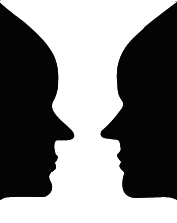
\includegraphics[scale=0.5]{img/twofaces.png}

\vspace{3cm}

\textit{Acknowledgements}\\
...


\end{center}


\pagebreak

\vspace{10cm}
\begin{center}
\textit{Please note}\\
Throughout this document, error bars show one standard error of the mean.\\
When discussing accuracy, we use both the $[0,1]$ interval and the $[0\%,100\%]$ interval. Thus a drop in accuracy of 0.03 is a drop of 3 percentage points.
\end{center}

\pagebreak

\tableofcontents

\pagebreak

\section{Introduction}


\section{Thesis organisation}

This document is organised into the following sections:

\section{Literature review}

\section{Terms}

\section{The overall goal}


\section{Modularity}

The property of modularity is the possibility to divide a system into multiple components!

\section{Forms of neural coding}

\begin{itemise}
\item \textbf{Single neuron activation}. The firing of a single neuron can convey binary information.
\item \textbf{Single spike frequency} can code a real-valued quantity.
\item \textbf{Spike frequency across multiple neurons} can code relative information between two real-valued quantities.
\item \textbf{Connection patterns} between neurons (the existence of a connection, or its strength) can code complex information, but this information cannot be extracted without activating the neurons and monitoring the outputs.
\end{itemise}

\section{Static and dynamic faces are processed differently}

The first evidence of a difference in the perception of expression between static and dynamic faces was found in 1991\cite{humphreys1993expression}.


\section{Identity vs. expression}

There is a substantial body of evidence that identity (information which is invariant within individuals) and expression (information which is invariant across perceived emotional states) are processed differently. On the high level, identity judgement and expression judgement have been observed to be doubly dissociated in prosopagnosics\cite{archer1994movement}. However, this observation may not allow us to generalise deductions to the normally-functional population, as prosopagnosics may have developed alternative recognition strategies such as non-holistic feature recognition (as is used to recognise classes of objects for which we do not possess a specialised representation or processing system).

On a slightly lower level, judgement reaction times differ depending on whether expression or identity is being judged; when judging identity, familiar faces are matched faster, but familiarity confers no advantage when judging expression\cite{bruce1986understanding}. This could imply that the computation of identity is intrinsically more complex or that other neural actions such as memory retrieval of biographical data are triggered.

On the lowest level, it is possible to find individual neurons which are receptive to either identity or expression\cite{hasselmo1989role}. Multidimensional scaling methods on their spike train data allow stimuli to be classified in either identity or expression space solely by neural response.

However, the location in one test subject of a small number of individual neurons which correlate with a particular condition provides no information about the algorithmics of face processing; it simply demonstrates that the brain can judge identity and expression at some level (which is intuitively obvious) and that this information can be coded by neural activation as opposed to connection patterning or higher-level codes such as spike train phase.

\section{Correlates between the two decouplings}

It is tempting to connect the identity-expression dichotomy with the static-dynamic dichotomy, as dynamic faces have constant identity but changing expression. This would be erroneous, as static faces can vary in both expression and identity.

\section{Object perception}

\section{Visual perception as dimensionality reduction}

Visual perception creates percepts from visual input. Photons arrive on the retina and induce signals in the optic nerve, which then pass to the LGN, dorsal and ventral visual pathways, and eventually effect conscious perception (such as when we perceive a face) or motor control (such as when we press a button to indicate that we have seen a face).

The number of photons arriving per unit time is so high that they cannot all be losslessly recorded, as shown by the reduced information capacity of the optic nerve\cite{wolff1993computing} compared to the retina, so information is compressed before dispatch. Motion representations are a simple form of compression; rather than recording the positions of a dot at each time-step (1,2,3,...,99,100), we can simply record its initial position (1) and speed (1 unit per second). Averaging is another simple compressor, as is nonlinear activation of cone cells (which require several afferent photons to change their membrane potential).


The bandwidth of the optic nerve is also smaller than that of incoming light signals, and this is dealt with by retinal adaptation.

%Insert from adaptation book here

These forms of compression can all be seen as transfer functions from low- to higher-level representations. The ultimate low-level representation of visual input is to record every photon arriving on the retina, but as this is impractical, optic nerve representations are compressed.

The process continues as we move further away from the retina and into the early visual system. Colour perception is another compression strategy, allowing any combination of wavelengths to be described by three coordinates in colour spaces like RGB, HSV or LAB.

Compression is evident in Marr's theory of vision, as in \cite{marr1978representation}:

"A representation is a formal system for making explicit certain entities or types of information, together with a specification of how the system does this. And I shall call the result of using a representation to describe a given entity a description of the entity in that representation."

Provided that Marr's "result" contains less information than his "entities or types of information," representation is precisely a process of compression.

Different types of representation record and miss different types of information. For example, neurons in V5 are sensitive to motion but not to colour; neurons in FFA are sensitive to faces but not houses. Many early visual centres are retinotopically mapped, keeping account of the position on the retina of a stimulus. This information, however, is not always useful: maintaining a map requires separate channels for each part of the visual field, even those which are not of interest.

In a retinotopically-mapped representation, it is easy to compare objects in the same position by simply subtracting or Pearson-correlating the corresponding areas. However, if the same object is present in the top-left of map A and the bottom-right of map B, comparing the two maps will not detect object identity.

In reality, object recognition is position-invariant: we are able to track an object as it moves around on the retina, and also to compare objects in different positions in the map. How position-invariant representations are built is a key problem in understanding the brain\cite{stringer2000position}.

Position-invariance is an important quality of object percepts, but is it sufficient to say that something is perceived as an object? Object perception is often associated with two other properties: spatiotemporal extent, and a canonical coordinate frame.

\paragraph{Spatiotemporal extent}
Most objects have spatial extent: defined borders. Prominent work on segmentation\cite{kiper1996cortical,grossberg1987role,atkinson1992visual,riseman1977computational,li1999visual} and figure-ground separation\cite{kelly2000neural,grossberg1993figure,grossberg19943} (which is simply segmentation from the background) underlines how important this process is to vision. Segmentation is task-specific: although we \textit{can} segment this object:
\begin{center}
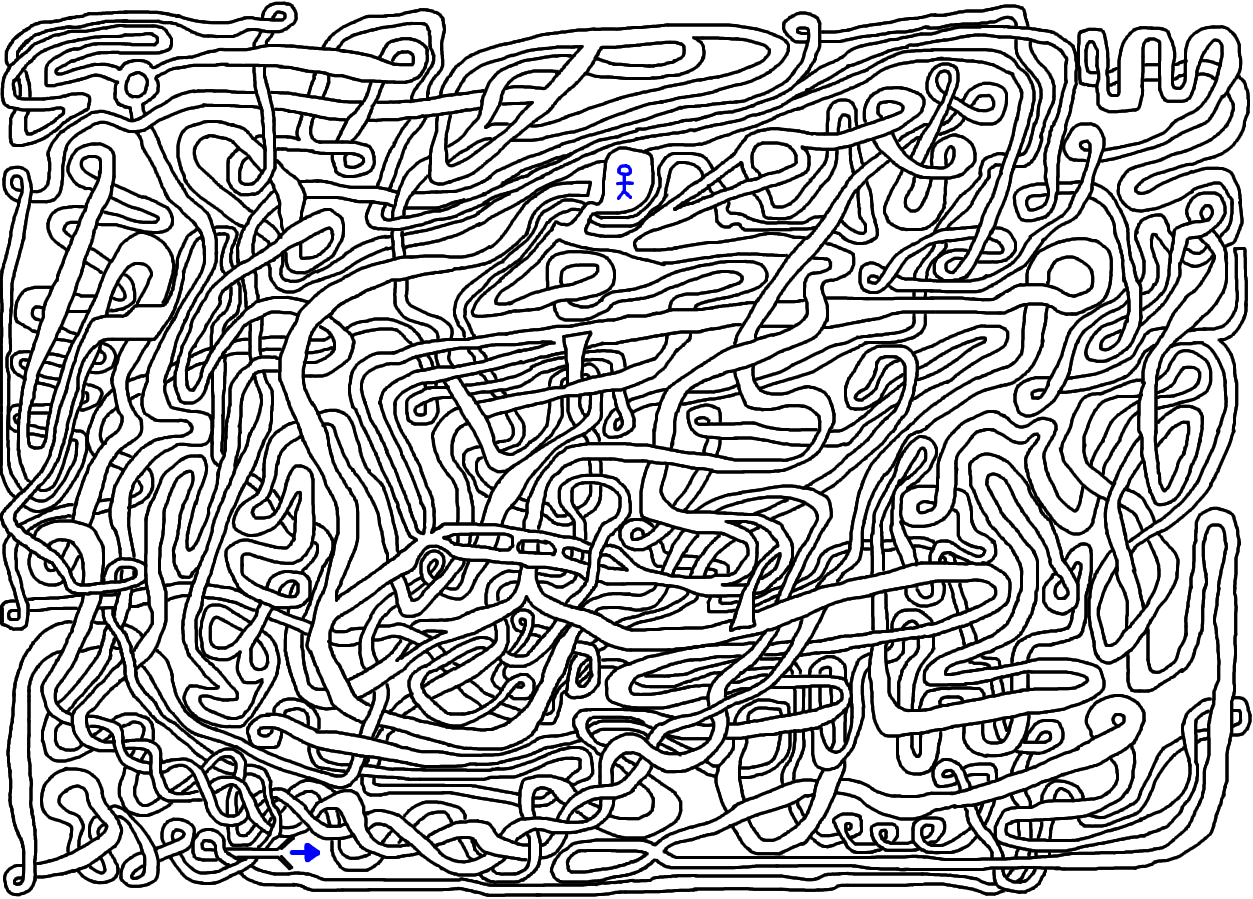
\includegraphics[width=0.3\textwidth]{img/maze.png}
\end{center}

we do not automatically perform that complex computation (and cannot without scanning the fovea over the image, as it is too detailed) unless engaged in a task which requires it, like copying the object.

When reasoning about dynamic stimuli, some objects have temporal extent: they appear at a certain moment, then disappear. Temporal extent is often task-sensitive. For example, a changing traffic light can be seen either as three permanent ``light" objects which change colour, or as ``red-light", ``yellow-light" and ``green-light" objects which appear when they illuminate and disappear when they darken.

\paragraph{Canonical coordinate frames}

Translation is not the only transformation under which objects are invariant: they also preserve their identity under 2D or 3D rotation and scaling. Marr pointed out that many objects are more easily recognised from certain points of view and inferred that they possess principal axes\cite{marr1982vision}. This property allows different objects of the same class to be compared; their principal axes can be aligned, allowing features to be registered.

In summary, objects are percepts which admit position invariance and have defined extent. However, all visual input is not segmented into objects. One of the main stimulus classes which we do not segment consists of textures.

\subsection{Textures}

There is much work on texture perception\cite{}, individuation\cite{} and classification\cite{}

Textures differ from objects 

\section{Representations}

It is important to note that there is never a unique representation of a visual stimulus, and it makes no sense to speak of "the" representation of a face or a house. Representations of a scene include:

Retinal photon trace (similar to a digital camera image)
Optic nerve representation
Neural recordings from V1
Neural recordings from the FFA
A verbal description of a scene
A written description of the scene

In terms of size, representations range from the very small (a recording from a single face-sensitive neuron can be taken to represent the presence or absence of a face in its receptive field) to the very large (such as Gallant's reconstruction of visual input from multivoxel MR imaging\cite{naselaris2009bayesian}).

The Marrean view sees representations as processes. Like other processes, such as functions, they can be composed so that information flows through them sequentially. Visual information flows from the retina to a single face-sensitive neuron as follows:

Retina - optic nerve - visual centres - FFA - neuron of interest

\subsection{Levels}

Representations can be seen to operate on different levels. We say that we move "up" from a low-level representation (the retina, or image space) to a high-level representation (FFA neurons, or face space). "Top-down control" indicates that cognitive representations accessible to consciousness are influencing low-level representations like motor neuron activity.

This up-and-down metaphor is very imprecise, despite being very common in the literature (over 369,000 results for the search "top-down control vision" on the Google Scholar literature search engine). It can generally be interpreted in two ways.

\paragraph{1. Top-bottom as distance from consciousness}
This view sees representations as being organised according to their interaction with consciousness. Qualia, intentions and percepts are the most high-level representations, as they are consciously accessible. Early visual system representations are seen as lower-level as they can be hidden from consciousness by processes like masking, crowding and adaptation. We refer to this as the \textbf{awareness scale}.

\paragraph{2. Top-bottom as representational information}
This view sees representations as being organised according to their information content, or entropy. Consider our two alternative codes for the 1D positions of a moving point, R1:(1,2 3,4,...,99,100) and R2:(start=1, speed=1). Although they describe the same thing, R1 contains 50 times more information than R2 (100 numbers compared to 50). We refer to this as the \textbf{information scale}.

These two metaphors describe completely different things, yet are mixed under the monikers "top-down" and "bottom-up." It is necessary to be very clear about which one we mean.

\subsection{Operations on representations}

Matching. Two representations can be compared for identity. This usually happens on two representations of equal information level





part_
\chapter{Experiments on fire alone}

\section{Recording and processing of stimuli}

A continuous 45-minute recording was acquired from a hearth fire using a Sony INS camera recording at 50 Hz. The scene was lit by a mixture of natural and artificial light and CCD gain was set to zero. Video was saved directly to the compressed AVCHD format at an initial resolution of 1024 by 768.

Before presentation, stimuli were cropped to 564 by 641 pixels, removing the background and most of the fireplace. Individual frames were decompressed and saved as bitmaps. 



\begin{figure}[htp]
\centering

\begin{subfigure}[b]{\textwidth}
\centering
                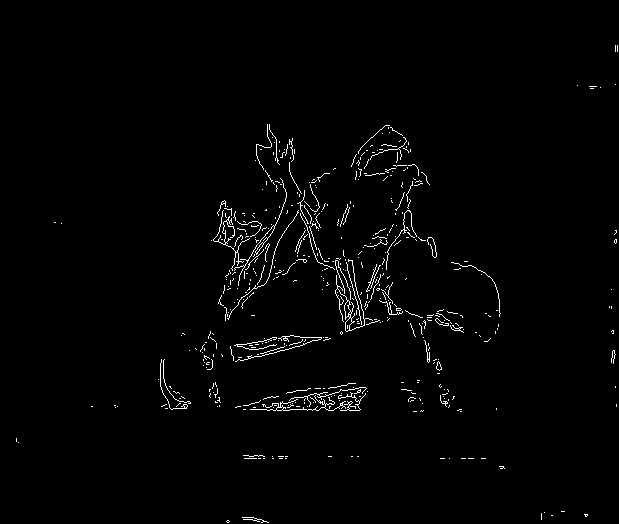
\includegraphics[width=12cm]{img/frame00000.png}
                \caption{Stimuli in original 1024 by 768 resolution.}
          
        \end{subfigure}

\begin{subfigure}[b]{\textwidth}
\centering
                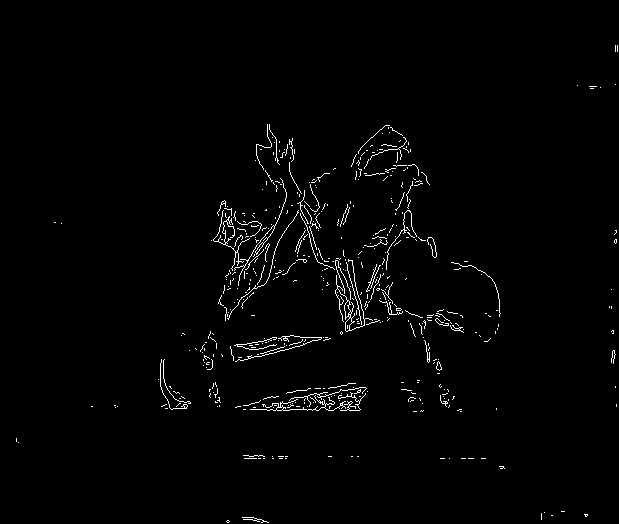
\includegraphics[width=12cm]{img/frame00000.png}
                \caption{Stimuli cropped to 564 by 641 pixels, as presented to subjects.}
          
        \end{subfigure}

\caption{Stimuli used in our visual search experiments.}
\end{figure}

\section{Experimental set-up}

Experiments were coded in MATLAB using Psychtoolbox. Video was displayed by loading bitmaps into video memory and manually displaying each one to the screen. This allowed precise control of frame rate.

Stimuli were displayed at 50 Hz on an INS monitor with a refresh rate of 100 Hz and a resolution of INS. The active video area subtended a visual angle of 14º; subjects used a chin-rest at a distance of 57 cm from the screen and were asked not to deviate their head angle from the vertical. Subjects were not requested to fixate, and the experiment took place in a darkened room.

All monitors used during these experiments were identically calibrated using a Cambridge Research Systems ColorCal or ColorCal MKII.


\section{Experiment 1: \textbf{search-ratio}}

\subsection{Methodology}

\paragraph{Stimuli}

A 1000-frame corpus of consecutive fire images was used.

\paragraph{Subjects}

12 subjects were recruited using a mailing list operated by University College London. All reported normal or corrected-to-normal vision.

\paragraph{Trial structure}

In each trial, a sample was presented first, followed by two tests. Subjects indicated which test they thought corresponded to the sample using the left arrow (first sample) and right arrow (second sample) keys. 

\paragraph{Factors}

Sample length (sL) was one of (10 25 50) frames, equivalently (0.2 0.5 1) seconds.
Ratio of sample to test was one of (1.2 1.4 1.6 1.8 2).

This gave the following sample lengths:
10-frame sample: 12 14  16 18 20 frames, 0.24, 0.28, 0.32, 0.36, 0.4 seconds
25-frame sample: 30 35 40 45 50 frames, 0.6,0.7,0.8, 0.9, 1 seconds
50-frame sample: 60    70    80    90   100 frames, 1.2,1.4,1.6,1.8,  2 seconds

There were 3*5 = 15 conditions.

\paragraph{Block structure}

25 training trials were presented first.

Sample length was varied across blocks. Target length was varied within blocks.

We presented 3 blocks, one corresponding to each target length, in random order. Subjects took a short break between blocks.

We used a total of 600 trials (40 trials per condition).

\subsection{Results}

\paragraph{Sample length}

We observed the following mean accuracies:

\begin{center}
\begin{tabular}{ r | l   }
\textbf{Sample length} & \textbf{Mean accuracy}\\
\hline
10 frames (0.2 s) & 0.728\\
 25 frames (0.5 s)&  0.704\\
 50 frames (1 s)&  0.687\\
\end{tabular}
\end{center}

Paired-sample $t$-tests revealed a significant accuracy drop between the 0.2 s samples and the 1 s samples ($p$<0.05) but not between any other pairs of levels. Subjects are more capable of matching longer samples.

\paragraph{Test/sample ratio}

The ratio by which the test was longer than the sample (which rises as the search space increases) had a significant effect on subject performance.

\begin{center}
\begin{tabular}{ r | l   }
\textbf{Test/sample ratio} & \textbf{Mean accuracy}\\
\hline
1.2 &  0.746\\
1.4 &  0.724\\
1.6 & 0.704\\
1.8 &  0.696\\
 2&  0.664\\
\end{tabular}
\end{center}

Paired-sample $t$-tests revealed significant differences between ratio=1.2 and each of the other levels; between ratio=1.8 and ratio=2 ($p<$0.05); and between ratio=1.4 and ratio=5 ($p<$0.01).

\paragraph{Learning rate}

We measured the subjects' learning rate by arranging the correct/incorrect responses in the order in which they were presented during the experimental run, blocking them into sequential groups of 20, and calculating the mean accuracy of each group. As shown in Fig. \ref{f:e1:learn}

\subsection{Discussion}

A two-factor repeated-measures ANOVA shows a highly significant effect of test/sample ratio ($p<$0.0001) but not of sample length ( ($p=$0.203) or of the ratio/sample length interaction ($p=$0.503). Neither is there an effect of absolute test length: see Fig. \ref{f:e1:tests}. The three sample length conditions ranged over three sets of test lengths which did not overlap at all; but, when re-expressed in terms of ratios, the effects on accuracy were consistent.

It is therefore the ratio between test and sample which determines the difficulty of the task\footnote{We use difficulty here as a proxy for accuracy, not to indicate the perceived ``hardness" of the task, which we did not measure.}, not the absolute lengths of either the target or the test.

 


\begin{figure}[htp]
\centering
\renewcommand{\arraystretch}{1.8}

      \begin{subfigure}[b]{\textwidth}
\begin{tabular}{ >{\bfseries}r | p{8cm}   }
& \textbf{Experiment 1}\\
\hline
  
	Design & 2AFC delayed match-to-sample (sample clip followed by two test clips)\\                   
  Stimuli & 1000-frame corpus \\
  Factors & sample length (10, 25, 50) frames or (0.2, 0.5, 1)seconds. \newline 
sample/test ratio (1.2 1.4 1.6 1.8 2).\\
  Block design & Sample length varied across blocks\newline
			Test length varied within blocks \newline
			15 conditions \newline
40 trials per condition \newline
600 trials \newline
25 training trials \\
\end{tabular}
\caption{Design summary.}
   \end{subfigure}

\begin{subfigure}[b]{\textwidth}
\centering
                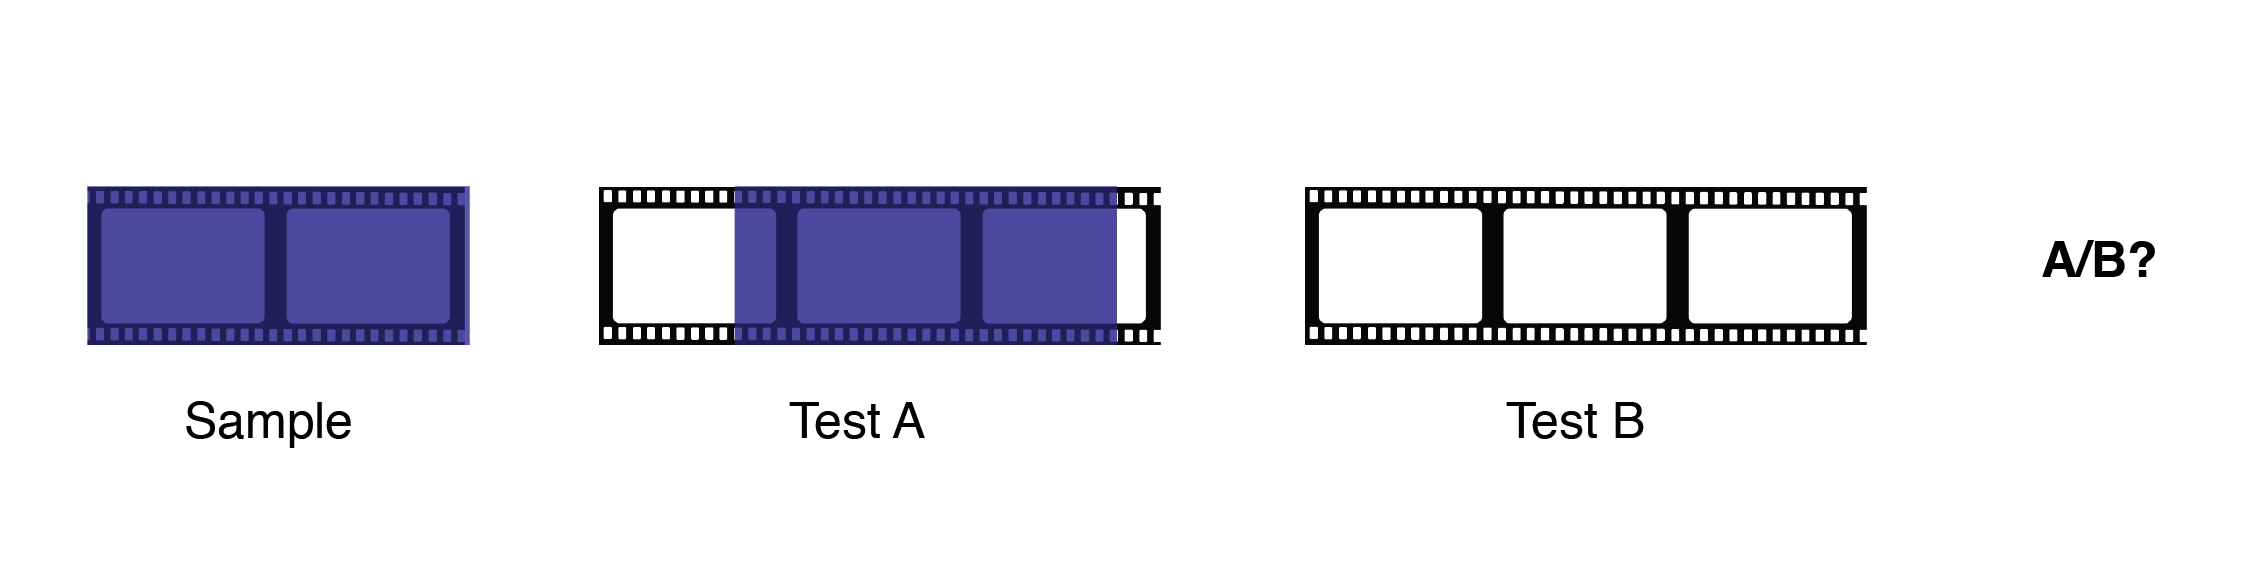
\includegraphics[width=12cm]{img/protocol_2afc.png}
                \caption{A short sample was followed by two longer tests, one of which contained the sample.}
         
        \end{subfigure}
\caption{Experiment 1: design summary and trial structure.}
\end{figure}


\begin{figure}[htp]
\centering
\begin{subfigure}[b]{\textwidth}
\centering
                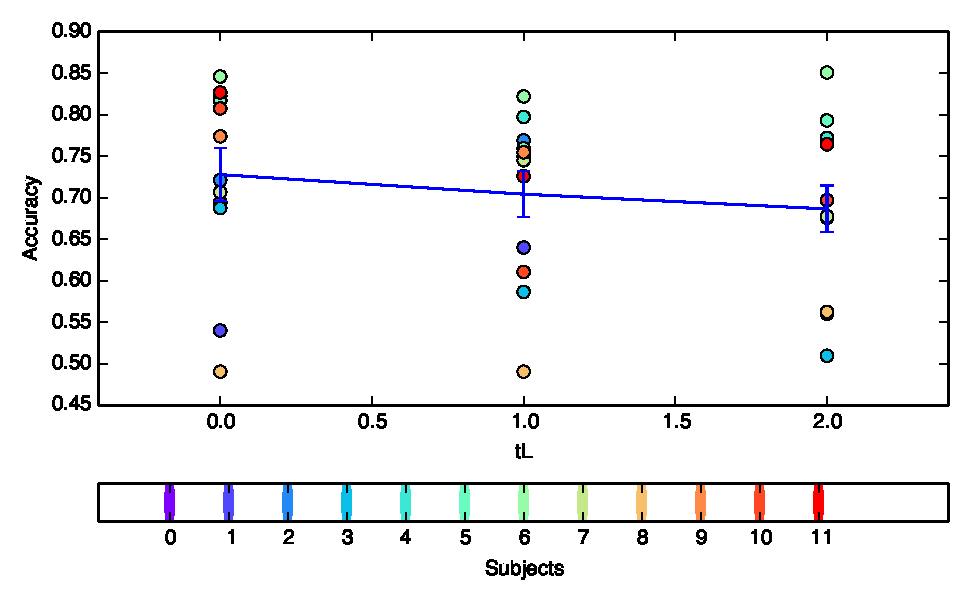
\includegraphics[width=12cm]{img/fig_fire3_correct_tL.pdf}
                \caption{Accuracy against sample length. Longer samples are more easily matched.}
          
        \end{subfigure}
\begin{subfigure}[b]{\textwidth}
\centering
                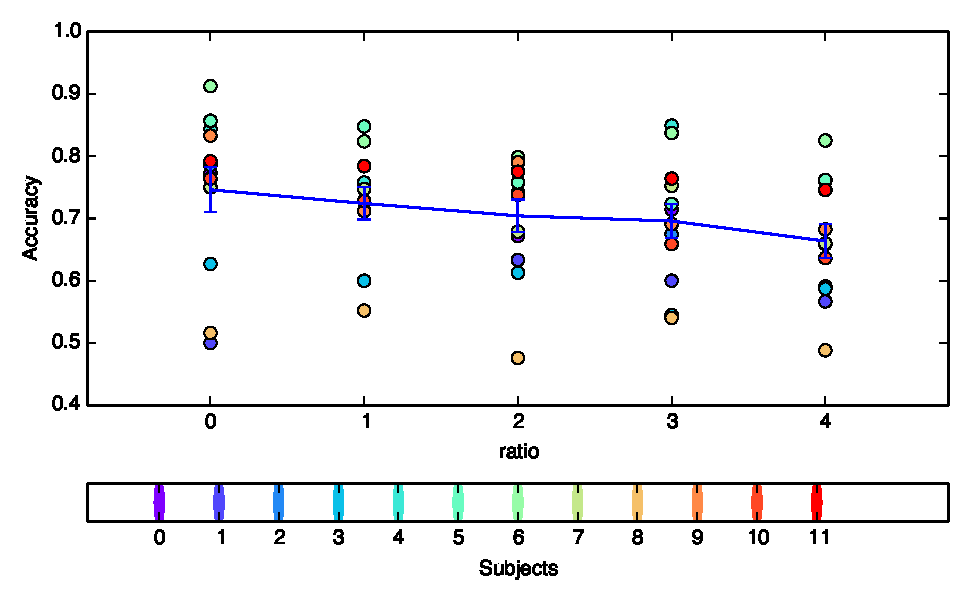
\includegraphics[width=12cm]{img/fig_fire3_correct_ratio.pdf}
                \caption{Accuracy against test/sample ratio. Longer tests render the sample harder to find.}
         
        \end{subfigure}
\caption{Experiment 1: the effects on accuracy of varying sample length, and test/sample ratio.}
\end{figure}

\begin{figure}[htp]
\centering
\begin{subfigure}[b]{\textwidth}
\centering
                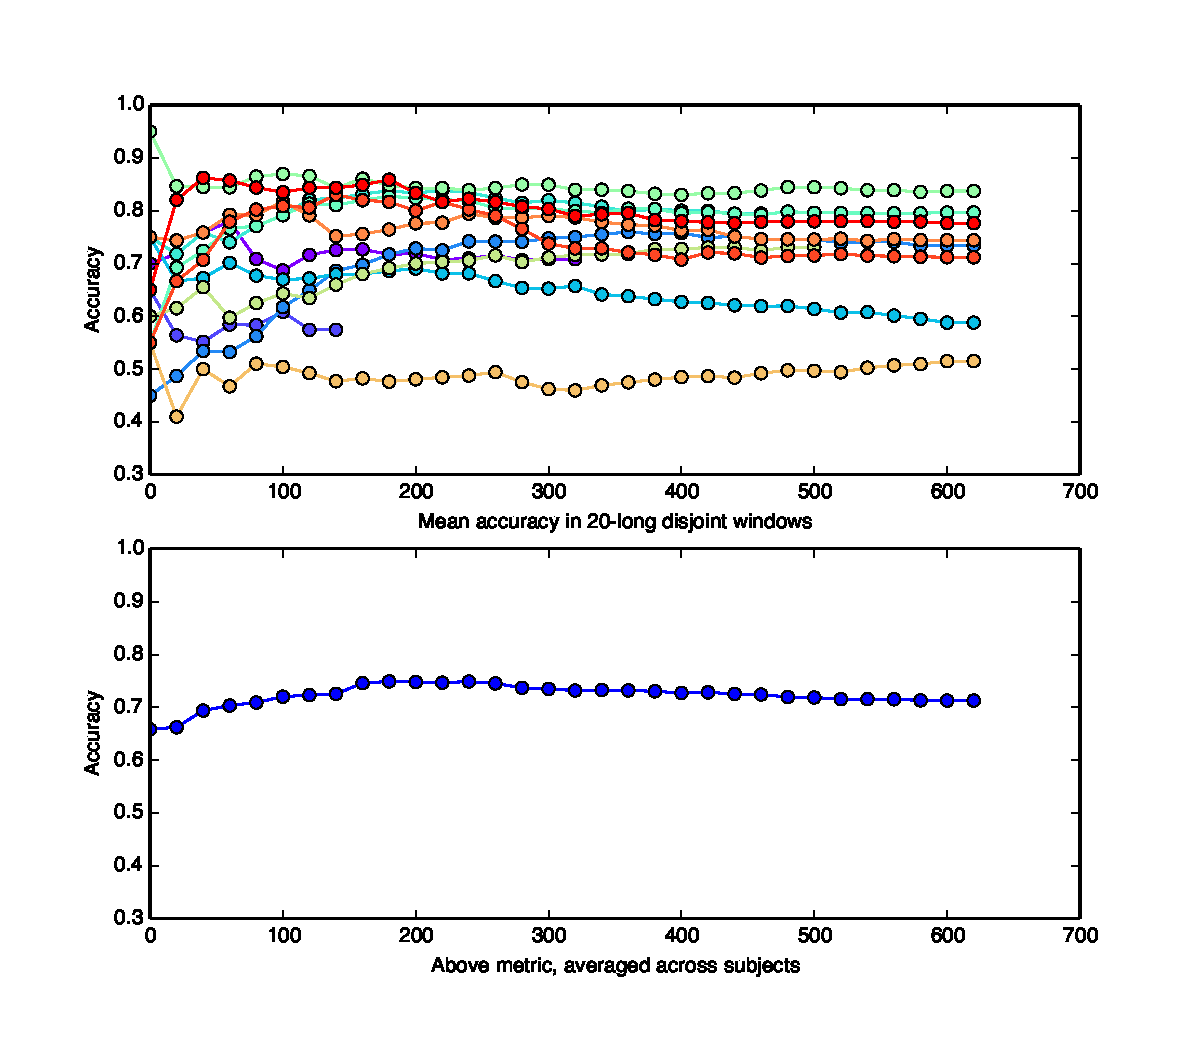
\includegraphics[width=12cm]{img/fig_fire3accuracyWalkingWindow.pdf}
                \caption{Learning: accuracy vs. trial number, blocked into groups of 20.}
      		\label{f:e1:learn}
        \end{subfigure}
\caption{Experiment 1: the effects on accuracy of varying sample length, and test/sample ratio. As throughout this document, error bars are 1 SEM.}
\end{figure}
\section{Experiment 2: \textbf{search-shortsamples}}


Experiment 1 showed us that the visual system can effectively discriminate the complex patterns of motion and form found in fire, but cannot effectively search for them in longer video sequences. However, it only looked at test clips between 0.2 and 1 seconds in length.

In order to look at the discriminability and searchability of shorter clips, we performed Experiment 2. This study used an identical 2AFC delayed-match-to-sample technique, but with shorter video clips lasting between 0.02 and 0.24 seconds (1 to 12 frames at 50Hz).

\subsection{Methodology}


\paragraph{Stimuli}

A 1000-frame corpus of consecutive fire images was used.

\paragraph{Subjects}

12 subjects were recruited using a mailing list operated by University College London. All reported normal or corrected-to-normal vision.

\paragraph{Trial structure}

In each trial, a sample was presented first, followed by two tests. Subjects indicated which test they thought corresponded to the sample using the left arrow (first sample) and right arrow (second sample) keys. 

\paragraph{Factors}

Sample length (sL) was one of (1, 3, 6, 12) frames, 
equivalently (0.02, 0.06, 0.12, 0.24) seconds.

Test length was one of (15,20,40) frames, equivalently (0.3,0.4,0.8) seconds.

There were 3*4 = 12 conditions. We presented a total of 480 trials (40 trials per condition).

\paragraph{Block structure}

24 training trials were presented first.

Test length was varied across blocks. Sample length was varied within blocks.

We presented 3 blocks, one corresponding to each test length, in random order. Subjects took a short break between blocks.

\begin{figure}[H]
\centering
\renewcommand{\arraystretch}{1.8}

      \begin{subfigure}[b]{\textwidth}
\begin{tabular}{ >{\bfseries}r | p{8cm}   }
& \textbf{Experiment 2}\\
\hline
  
	Design & 2AFC delayed match-to-sample (sample clip followed by two test clips)\\                   
  Stimuli & 1000-frame corpus \\
  Factors & sample length: (0.02, 0.06, 0.12, 0.24) seconds or (1, 3, 6, 12) frames. \newline 
sample/test ratio: (0.3,0.4,0.8) seconds or (15,20,40) frames.\\
  Block design & Test length varied across blocks\newline
			Sample length varied within blocks \newline
			12 \newline
40 trials per condition \newline
600 trials \newline
25 training trials \\
\end{tabular}
\caption{Design summary.}
   \end{subfigure}

\begin{subfigure}[b]{\textwidth}
\centering
                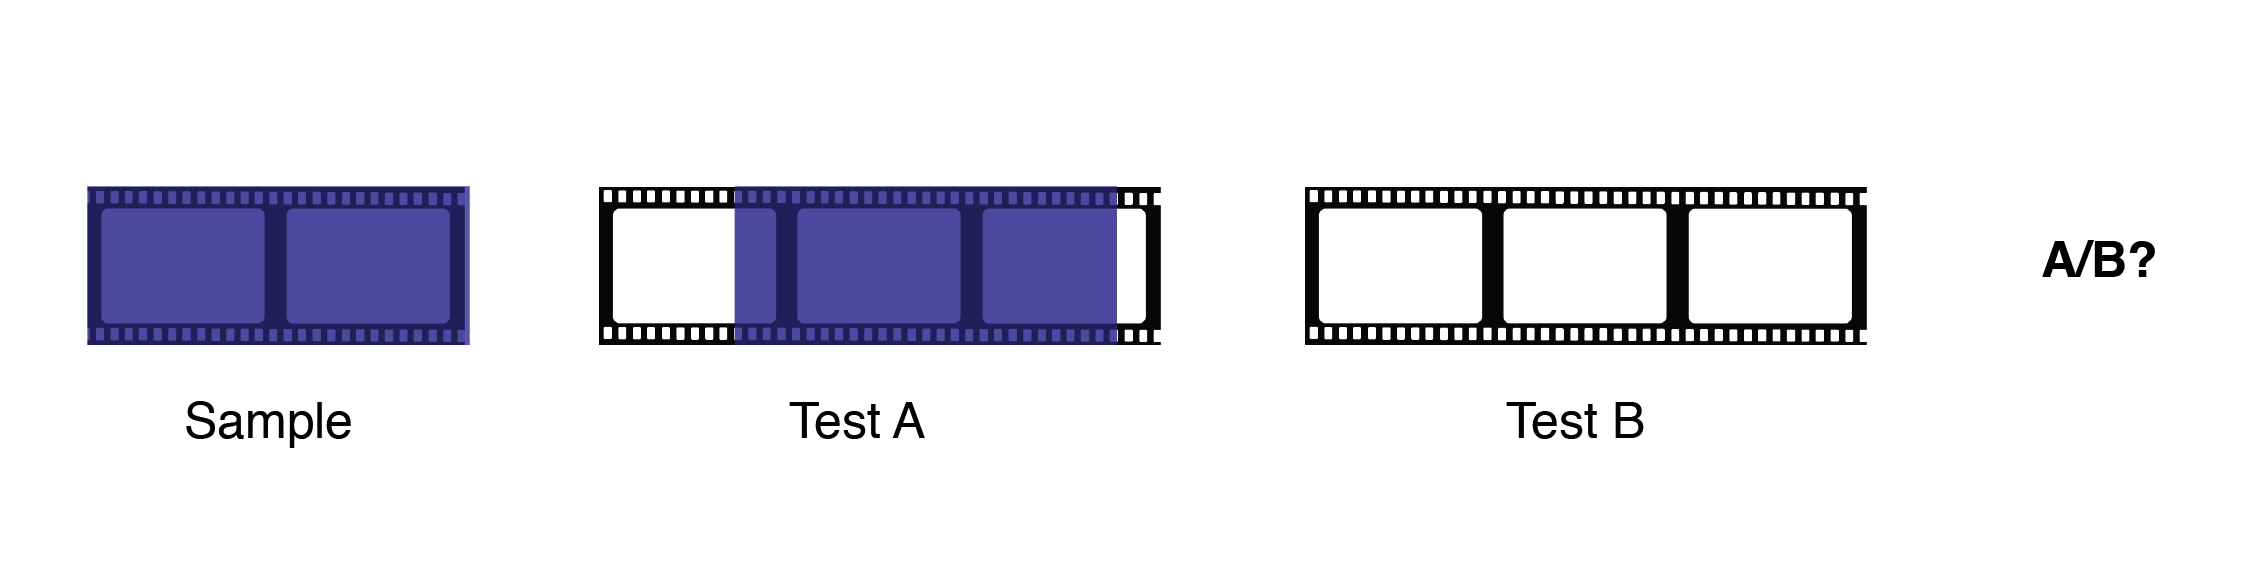
\includegraphics[width=12cm]{img/protocol_2afc.png}
                \caption{A short sample was followed by two longer tests, one of which contained the sample.}
         
        \end{subfigure}
\caption{Experiment 2: design summary and trial structure.}
\end{figure}

\subsection{Results}

\paragraph{Sample length}

Accuracy increased significantly with the length of the sample, and $t$-tests showed that it was always above chance across different sample lengths. Two-way repeated-measures ANOVA revealed a significant effect of sample length ($p<$0.00001), but not of test length ($p=$0.652), and no interaction between the two ($p<$0.395). Mean accuracies by target length were:


\paragraph{Learning}

As shown in Fig. \ref{f:e2:learn}, there is no discernible effect of learning during this task: subjects' accuracy did not improve during the first 100 trials, as in Experiment 1. It is tempting to explain this result by the fact that Experiment 1 kept sample lengths constant within blocks, allowing subjects to tune their mental set to a particular sample length. However, Experiment 1 used 3 blocks of 200 trials each, and we note no drop in accuracy after the end of the first or second block. We thus conclude that the lack of learning is related to the shorter sample lengths.

\begin{center}
\begin{tabular}{ r | l   }
\textbf{Sample length} & \textbf{Mean accuracy}\\
\hline
0.02 s &  0.6\\
0.06 s&  0.67\\
0.12 s& 0.70\\
0.24 s&  0.73\\
\end{tabular}
\end{center}

\begin{figure}[htp]
\centering
\begin{subfigure}[b]{\textwidth}
\centering
                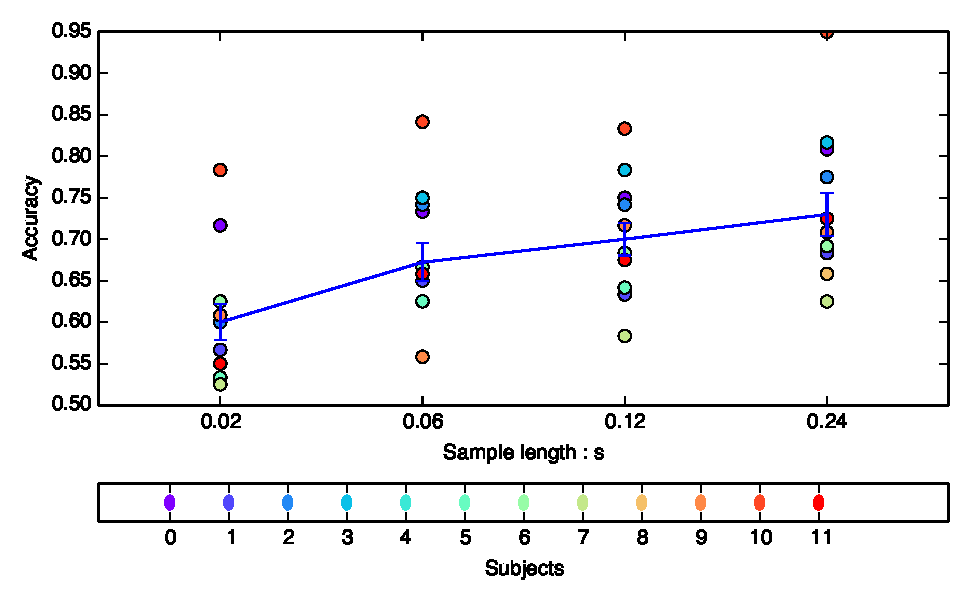
\includegraphics[width=12cm]{img/fig_fire4_correct_sampleL.pdf}
                \caption{Accuracy against sample length. Longer samples are easier to match.}
          
        \end{subfigure}
\begin{subfigure}[b]{\textwidth}
\centering
                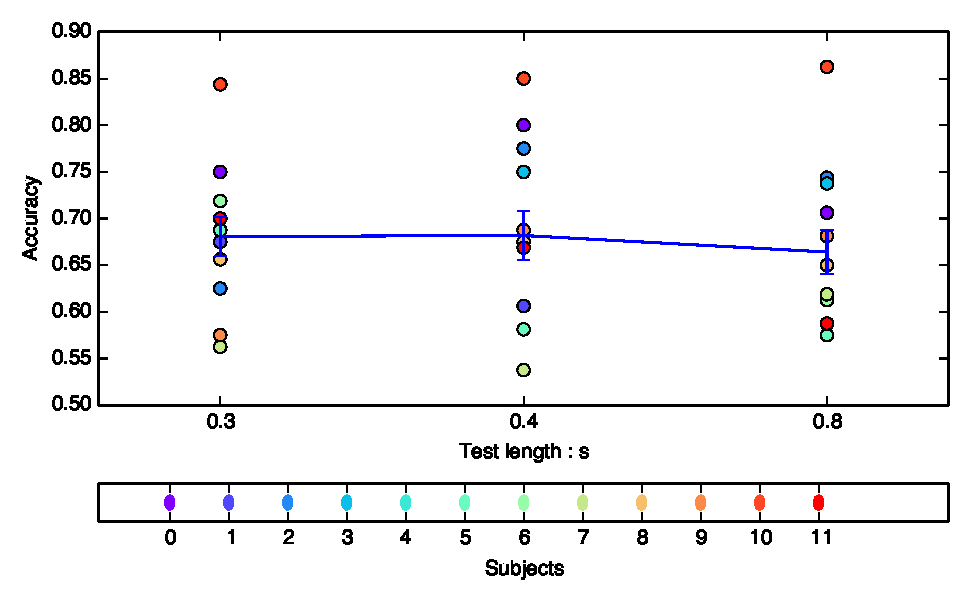
\includegraphics[width=12cm]{img/fig_fire4_correct_testL.pdf}
                \caption{Accuracy against test length. Search for samples under 0.24 seconds is not affected by test length.}
         
        \end{subfigure}
\caption{Experiment 2: For samples under 0.24 seconds, search is more effective with longer samples; however, test length makes no difference up to 0.8 seconds.}
\end{figure}

\begin{figure}[htb]
\centering
\begin{subfigure}[b]{\textwidth}
\centering
                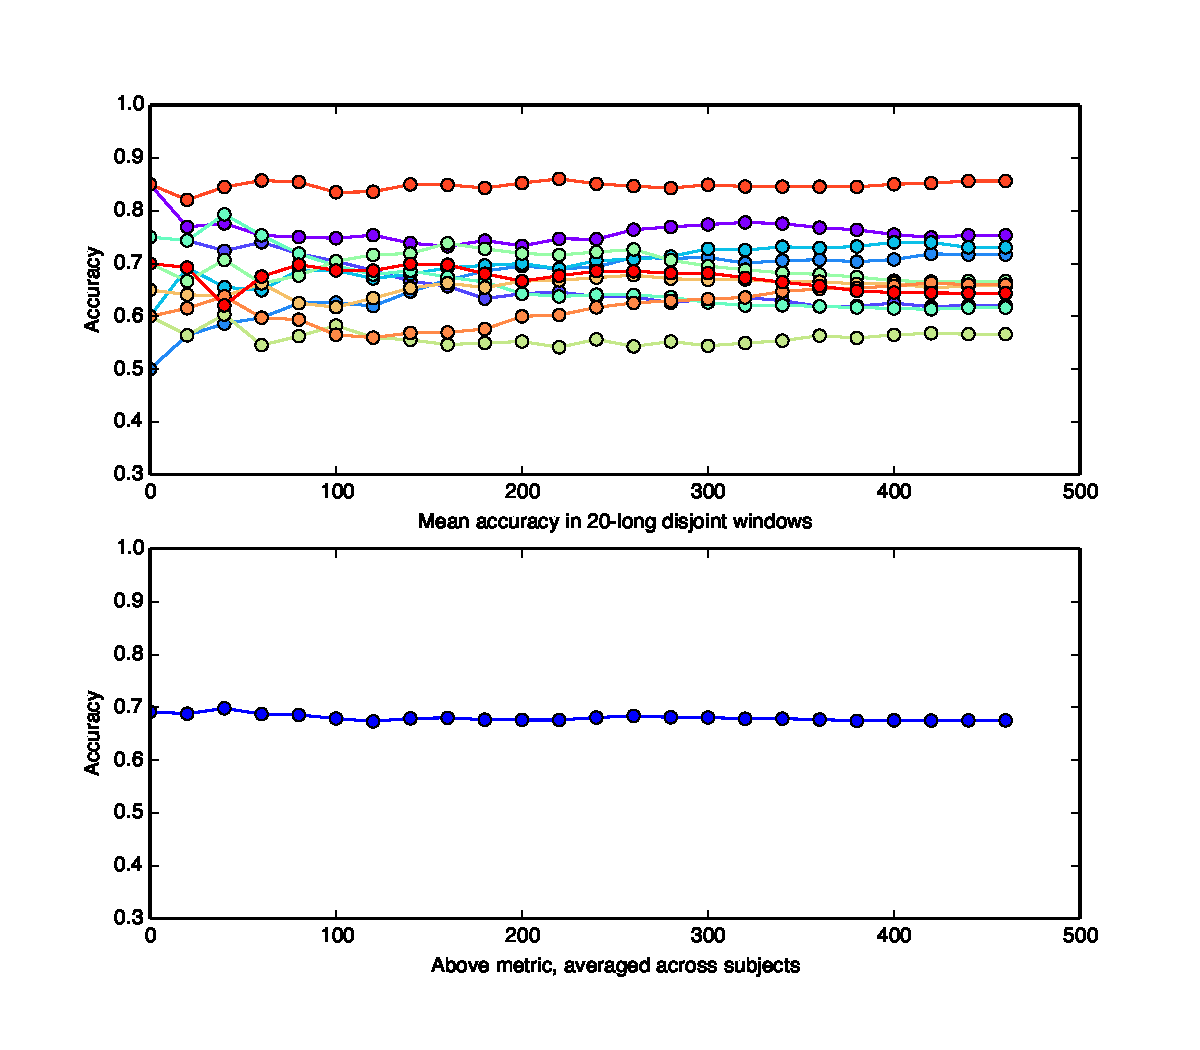
\includegraphics[width=12cm]{img/fig_fire4accuracyWalkingWindow.pdf}
                \caption{Learning: accuracy vs. trial number, blocked into groups of 20.}
      		\label{f:e2:learn}
        \end{subfigure}
\caption{Experiment 2: for short samples under 0.24 seconds, there is no discernible effect of learning.}
\end{figure}

\subsection{Discussion}
\section{Experiment 3: Visual search in more detail}

\subsection{Methodology}

\paragraph{Stimuli}

A 10,000-frame corpus of consecutive fire images was used.



\paragraph{Subjects}

11 subjects were recruited using a mailing list operated by University College London. All reported normal or corrected-to-normal vision.

\paragraph{Trial structure}

Yes-no delayed match-to-sample with altered sample.
In each trial, a sample was presented first, followed by a single test. Subjects indicated whether they thought the sample corresponded to the test (up arrow) or now (down arrow).

Samples were all one second (50 frames).

Test clips consisted of the sample, surrounded by a pre-clip and a post-clip, which could both be of length zero.



\paragraph{Factors}

The lengths of the pre-clip and the post-clip (which we term prelength and postlength) were picked from (0, 25,50,100) frames or (0, 0.5,1,2) seconds. Each factor thus had four levels, leading to 16 conditions.

\paragraph{Block structure}

We used 30 training trials with both samples and tests of length one second, and no pre-or post-clips.

The experiment was divided into 10 blocks; subjects took a break between each block. There were 40 trials per block (400 trials total). There were 16 conditions (4*4 factors) and 25 trials per condition.


\begin{figure}[H]
\centering
\renewcommand{\arraystretch}{1.8}

      \begin{subfigure}[b]{\textwidth}
\begin{tabular}{ >{\bfseries}r | p{8cm}   }
& \textbf{Experiment 3}\\
\hline
  
Design & 2AFC delayed match-to-sample, with filtered or inverted sample\\                   
Stimuli & 10000-frame corpus\newline
		1 second sample (50 frames)\newline
		variable-length test\\
Factors & prelength:\newline
		(0, 25,50,100) frames or (0, 0.5,1,2) seconds\newline
		postlength:\newline
		(0, 25,50,100) frames or (0, 0.5,1,2) seconds\newline\\

Block design & prelength and postlength varied within blocks\newline
		10 identical blocks\newline
25 trials per condition \newline
40 trials per block \newline
400 trials \\
Training &30 training trials \\
Subjects&11\\
\end{tabular}
\caption{Design summary.}
   \end{subfigure}

\begin{subfigure}[b]{\textwidth}
\centering
                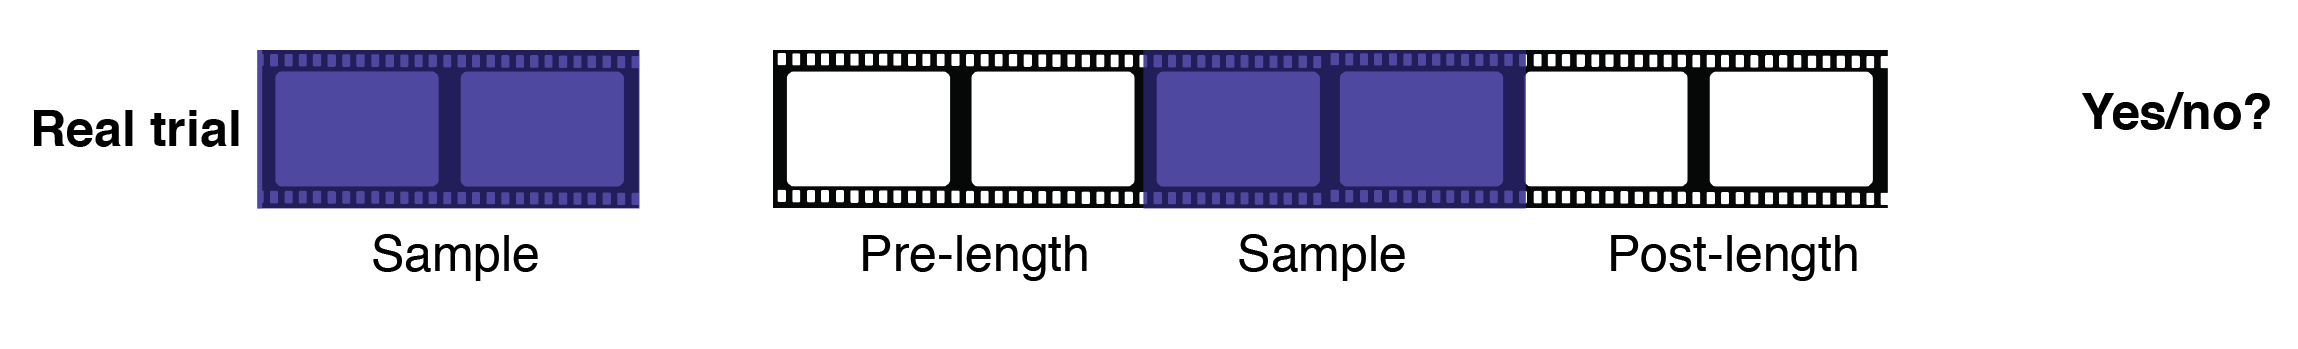
\includegraphics[width=12cm]{img/protocolfire18.png}
                \caption{An altered (filtered or inverted) sample was followed by two untouched tests, one of which contained the sample.}     
        \end{subfigure}
\caption{Experiment 3: design summary and trial structure.}
\end{figure}

\subsection{Results}

\paragraph{Prelength and postlength}

Prelength and postlength could only be defined for the true trials (tests in which the subject was present), not for the foil trials (tests in which the subject was absent).

Over the true trials, a two-way repeated-measures ANOVA revealed no significant effect of prelength or postlength.

\paragraph{Total distractor time and test presence}

The pattern of accuracy in function of total time was related to whether the test was present (true trials) or absent (foil trials). For true trials, accuracy first decreased and then increased as distractor length went up. For foil trials, accuracy smoothly decreased as distractor length went up.

In other words, as distractor length increased:
\begin{itemise}
\item Hits stayed high (with a slight down then up trend), and misses stayed low (with a slight up then down trend)
\item Correct rejects declined, and false positives increased
\end{itemise}

As search space increased, the source of errors is mainly due to false positives, not misses. Accurate judgements were mainly due to hits, not correct rejects. Observers were good at finding a present target, but tended to confuse an absent target for a present one.



\paragraph{Beginning trials and end trials}

We define beginning trials as true trials where the sample was present at the beginning of the test, and end trials as those where the sample was present at the end of the test. In the set of beginning trials, the trial counts by level of postlength were constant; similarly, in the set of end trials, the trial counts by level of prelength were constant. This provided a useful contrast to the analysis by totaltime, where there were neccesarily vastly different numbers of trials at each level.


\paragraph{Signal detection analysis}

As this was a yes/no experiment, we analysed the accuracy pattern using the framework of signal detection theory\cite{green1966signal}. 

First we calculated the collective $d'$ across all subjects for each level of total distractor time. The $d'$ curve followed the same shape as subject accuracy: first descending, then increasing as total time increased.

\paragraph{ROC analysis}

We plotted each subject in ROC space, the 2-$D$ space defined by hit rate over false positive rate\cite{flach2003geometry}.



\begin{figure}[htp]
\centering
\begin{subfigure}[b]{\textwidth}
\centering
                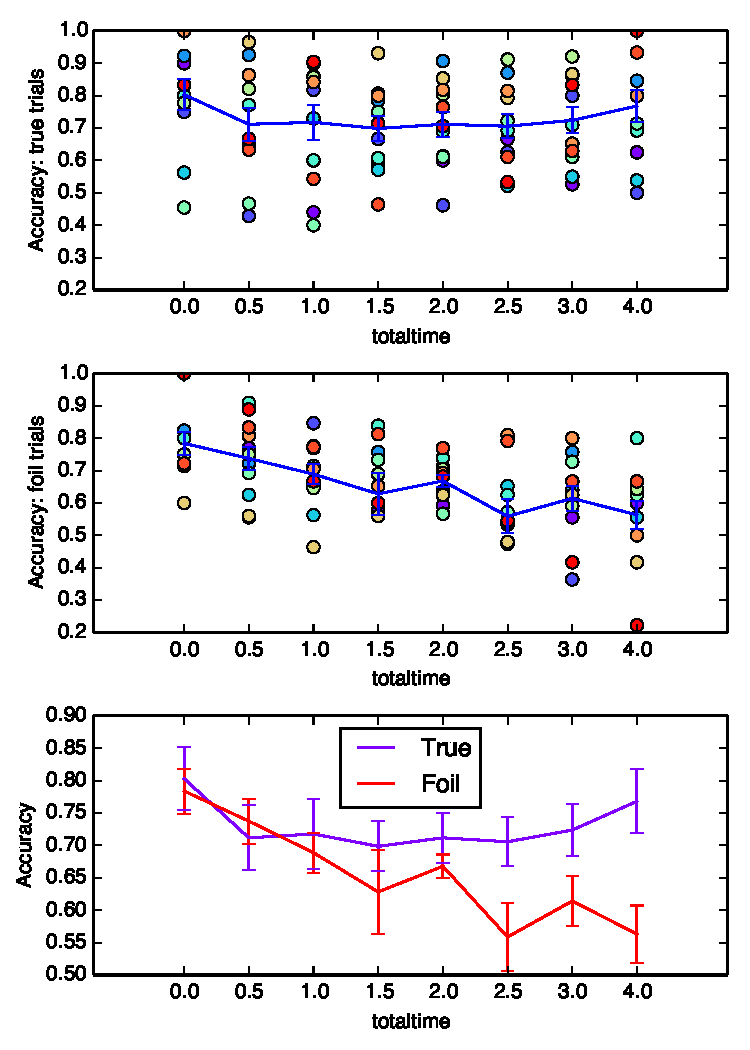
\includegraphics[width=12cm]{img/fig_fire18_totaltime_YN.pdf}
                \caption{Accuracy in function of the five manipulations.}
          
        \end{subfigure}


\caption{Experiment 3: Detection was above chance under all manipulations, but was too low to discern a contrast between the effects.}
\end{figure}

\subsection{Discussion}



Observers were good at finding a present target, but tended to confuse an absent target for a present one. This allows us to rule out a range of search systems: those where the choice of representation was independent of the features observed during the test.




\section{Experiment 4: the importance of edges}

\subsection{Methodology}

\paragraph{Stimuli}

A 1000-frame corpus of consecutive fire images was used.

\paragraph{Subjects}

15 subjects were recruited using a mailing list operated by University College London. All reported normal or corrected-to-normal vision.

\paragraph{Trial structure}

2AFC Delayed match-to-sample with altered sample.
In each trial, a sample was presented first, followed by two tests. A manipulation was applied to the sample; the tests were unchanged. Subjects indicated which test they thought corresponded to the sample using the left arrow (first sample) and right arrow (second sample) keys. 

Sample length (sL) was one 10 frames (0.2 seconds)
Test length was 15 frames (0.3 seconds)

\paragraph{Factors}

In half the trials, the sample was manipulated using a Sobel edge filter. The test clips were left unchanged.

Each frame was convolved with the 3x3 filter

    0.1250    0.2500    0.1250
         0         0         0
   -0.1250   -0.2500   -0.1250

to give an estimate of the image derivative. All pixels above a certain threshold value in the derivative image were returned as edges. The implementation used was MATLAB's edge() function.


\paragraph{Block structure}

Firstly, we presented 30 training trials with static samples and tests (displayed for 0.2 and 0.3 seconds respectively), half of which used the edge-filtered sample.

Next, we presented 15 training trials with dynamic samples and tests and the same clip lengths, but with samples and tests unaltered.

There were 2 block types; we presented each block 7 times (in random order), giving a total of 14 blocks.
We presented 40 trials per block, giving a total of 560 trials.


\begin{figure}[H]
\centering
\renewcommand{\arraystretch}{1.8}

      \begin{subfigure}[b]{\textwidth}
\begin{tabular}{ >{\bfseries}r | p{8cm}   }
& \textbf{Experiment 4}\\
\hline
  
	Design & 2AFC delayed match-to-sample (sample clip followed by two test clips)\\                   
  Stimuli & 1000-frame corpus \\
  Factors & sample edge-filtered or untouched \newline \\
  Block design & 14 blocks, half edge-filtered \newline
280 trials per condition \newline
560 trials \newline
45 training trials \\
Subjects & 15\\
\end{tabular}
\caption{Design summary.}
   \end{subfigure}

\begin{subfigure}[b]{\textwidth}
\centering
                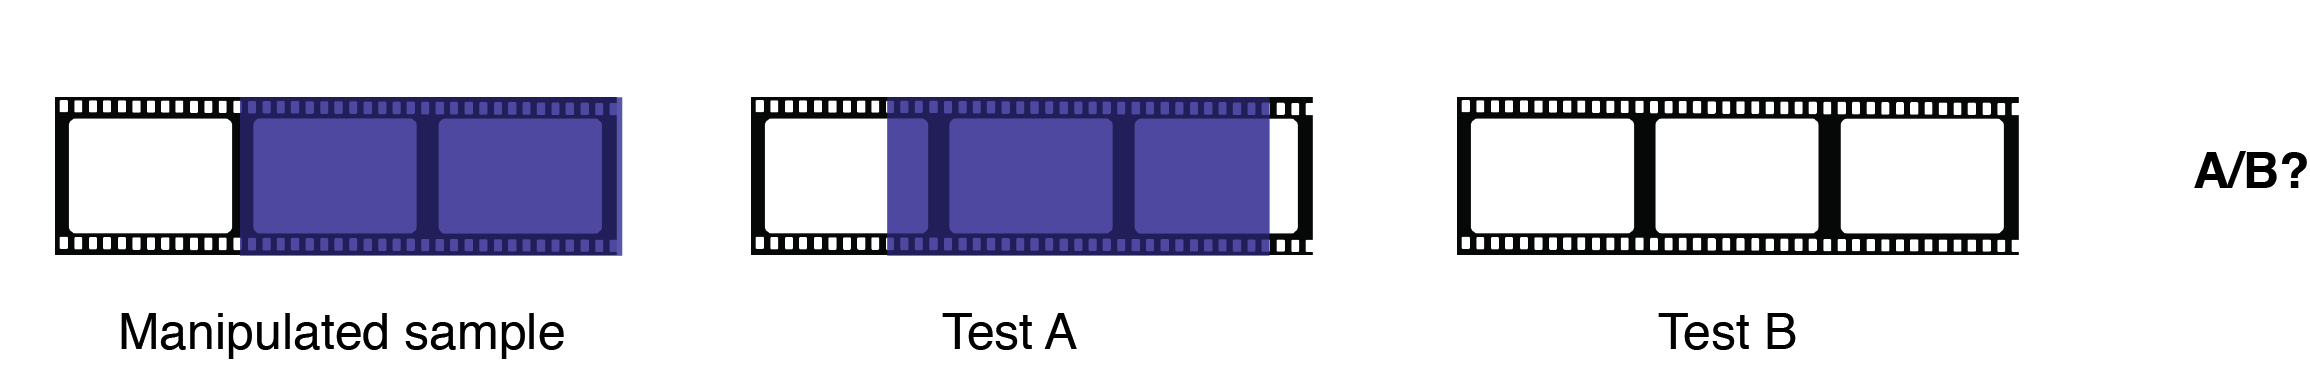
\includegraphics[width=12cm]{img/fire5protocol.png}
                \caption{A short sample was followed by two longer tests, one of which contained the sample.}
         
        \end{subfigure}
\caption{Experiment 4: design summary and trial structure.}
\end{figure}


\subsection{Results}

\paragraph{Edge filtering}

Edge-filtering the sample induced a 4 percentage point drop in accuracy compared to the normal condition:

\begin{center}
\begin{tabular}{ r | l   }
\textbf{Sample} & \textbf{Mean accuracy}\\
\hline
Normal &  0.782\\
Edge-filtered&  0.742\\
\end{tabular}
\end{center}


This difference was significant (paired-samples $t$-test, $p$<0.005).

\paragraph{Order}

Presenting the sample as the first test (as opposed to the second test) induced an accuracy drop of 4.5 percentage points:

\begin{center}
\begin{tabular}{ r | l   }
\textbf{Test order} & \textbf{Mean accuracy}\\
\hline
True test first &  0.785\\
Foil test first&  0.740\\
\end{tabular}
\end{center}

However a paired-samples $t$-test did not find this difference significant ($p$=0.22).




\begin{figure}[htb]
\centering
\begin{subfigure}[b]{\textwidth}
\centering
                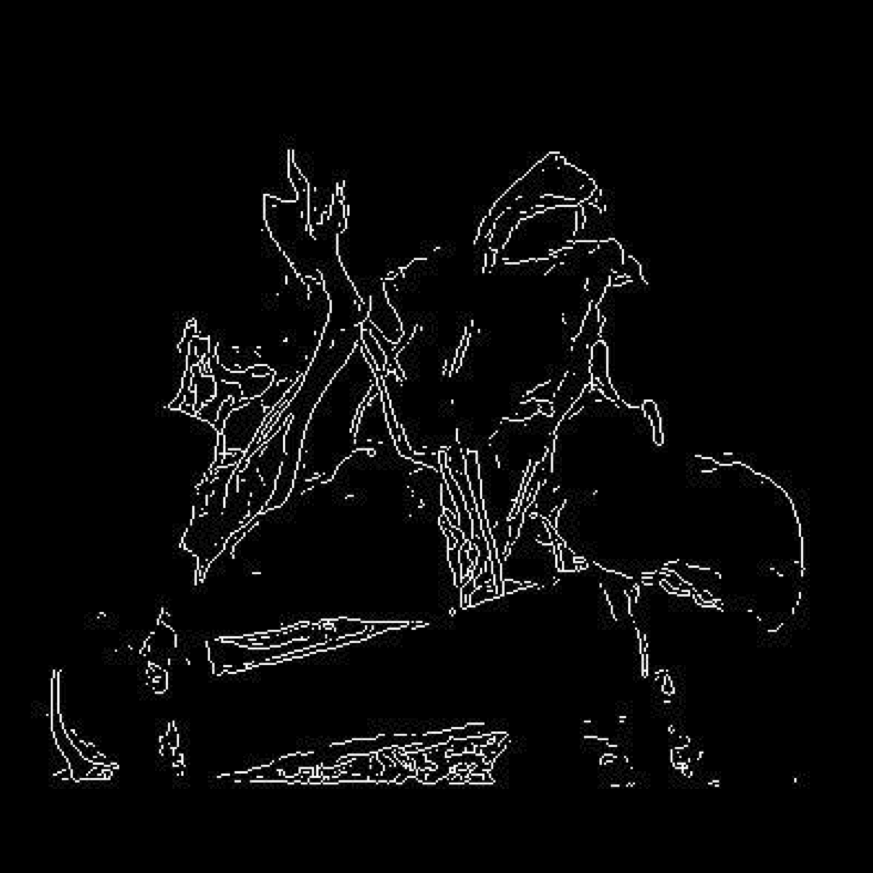
\includegraphics[width=5cm]{img/edges.png}\hspace{0.5cm}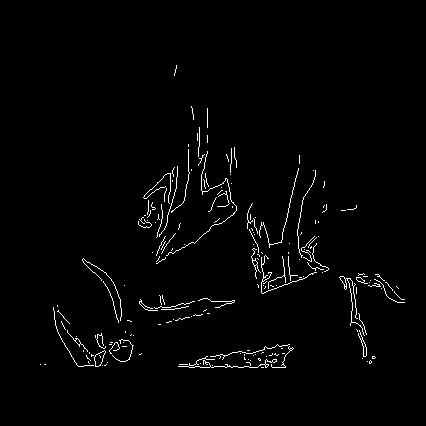
\includegraphics[width=5cm]{img/edges2.png}
                \caption{Two edge-filtered frames.}
         
        \end{subfigure}
\begin{subfigure}[b]{\textwidth}
\centering
                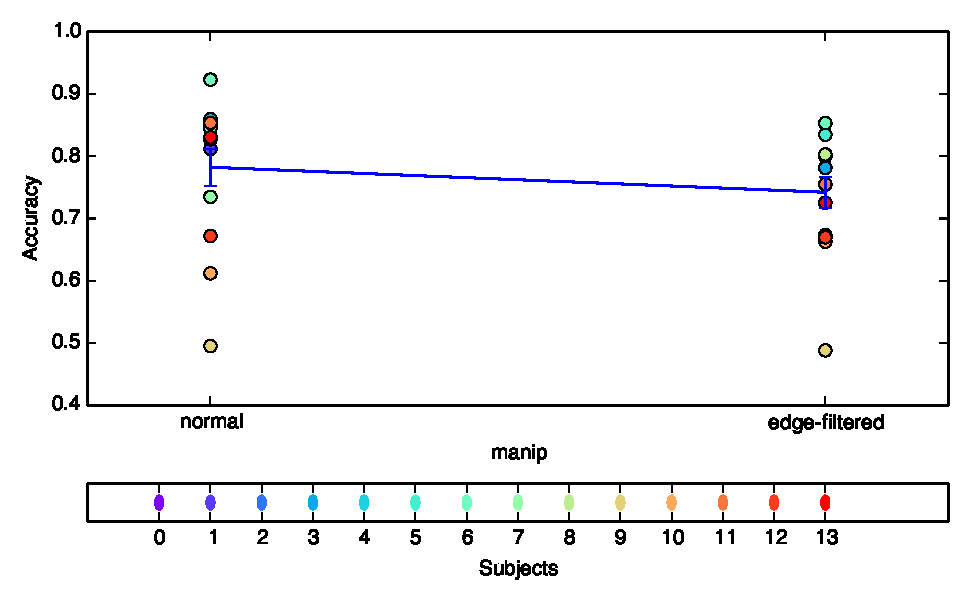
\includegraphics[width=12cm]{img/fig_fire10-edges_correct_manip.pdf}
                \caption{Edge-filtering the samples induced a 4 percentage point accuracy drop.}
      		\label{f:e2:learn}
        \end{subfigure}
\caption{Experiment 4: detecting a sample based on its edges alone.}
\end{figure}

\subsection{Discussion}


Edges are very important in the representation of fire. We are able to match a sample clip from which all of the texture and fine contrast information has been removed, with an unaltered test, with only a small impairment from normal performance. This shows that the visual system is able to extract very useful information from flame edges alone, and employ it effectively for comparison.

This observation allows us to reject the hypothesis that fire matching is done based on the global average luminance signal, which is not preserved under edge filtering.

Edges are very important in the generation of salience maps\cite{alter1998extracting}, which guide attention to features useful for discrimination. The generation of salience percepts is not local, as evidenced by its tendency to highlight features which form global shapes:

\begin{center}
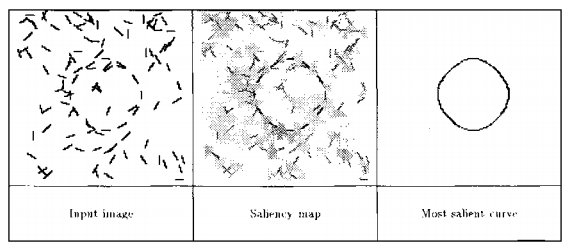
\includegraphics[width=0.7\textwidth]{img/salience}\\
\textit{The circle in the first image is detectable both by your visual system and by the Shashua and Ullman model described by this figure from \cite{alter1998extracting}.}
\end{center}

However, the edges in this experiment were generated purely locally, by convolving each frame with the matrix


\[
M=
  \begin{bmatrix}
    0.125 & 0.25 & 0.125\\
    0 & 0 & 0\\
-0.125 & -0.25 & -0.125\\
  \end{bmatrix}
\]

which is only 3-by-3 and thus very local. Edge detection has often been used as an input to saliency map generators, which are more global; one small object by itself in a large image is very salient, but when surrounded by dozens of similar objects, salience is quickly lost.

Salience-map calculation is related to grouping, but is quite different. We define grouping as the process by which local features are bound together into global features, as, for example, the local edge elements in the image just above are unified into the percept of a circle. It is often assumed that grouping, like salience, can be implemented by a map: a representation composed of local pixel-like elements in which each element is tagged with the identity of the object it belongs to.

There are several problems with this idea:

\begin{itemise}
\item Maps make sense for scalar quantities like luminance and salience, but object identity is not scalar: how do we code \emph{teapot} or \emph{face} in a scalar manner?

\item Maps do not make sense for hierarchical representations: one pixel of a human body can belong to \emph{finger}, \emph{hand}, \emph{arm}, \emph{upper body} and \emph{John}. There is no room in a map to code all of this information.

\item Object segmentation can be a very complex computation and is not always performed unless required. For example, in the following image, we can decide whether two points belong to the same object if asked:

\begin{center}
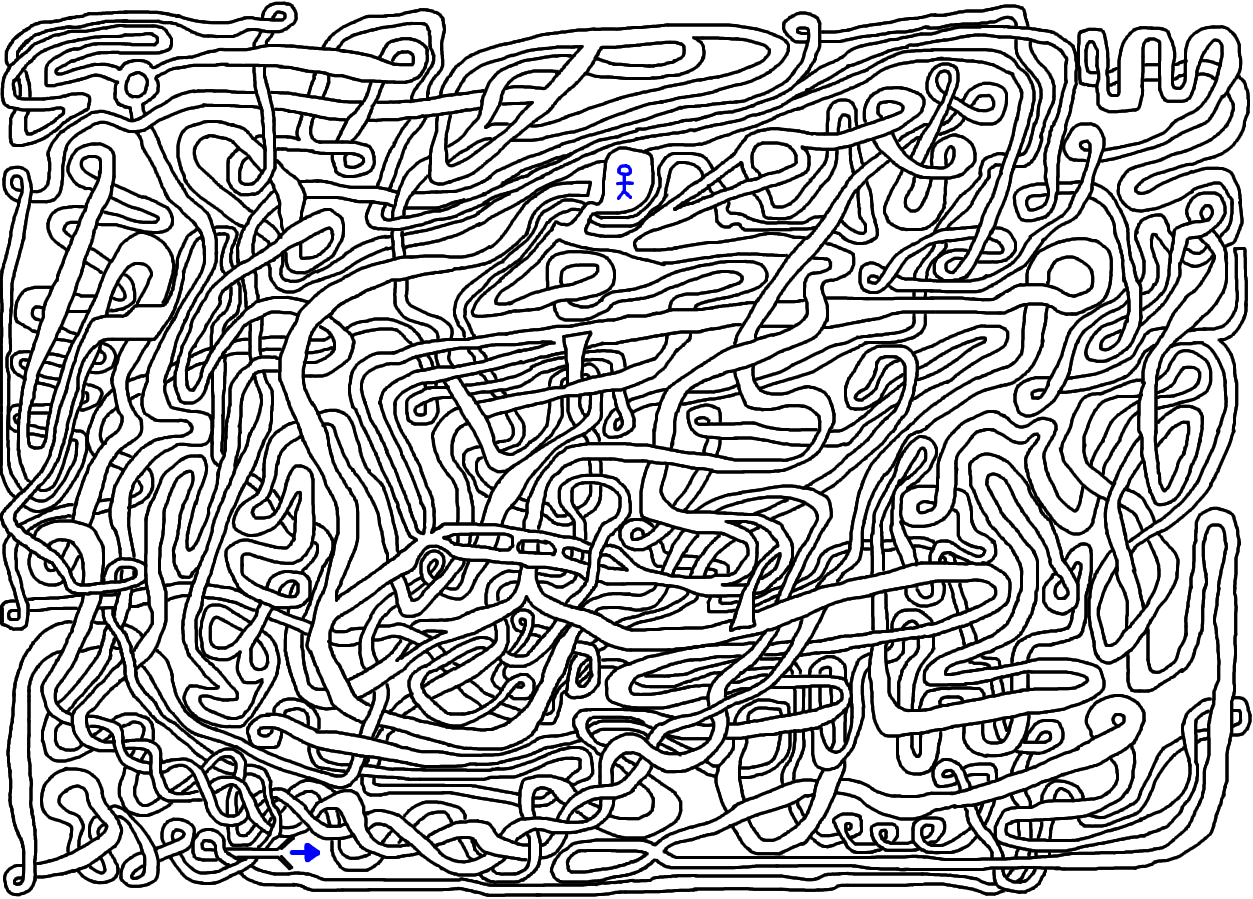
\includegraphics[width=0.4\textwidth]{img/maze.png}
\end{center}

but this computation is not performed in an automatic manner.

\end{itemise}

\section{Experiment 5: colour, inversion and reversal}

\subsection{Methodology}


\paragraph{Stimuli}

A 1000-frame corpus of consecutive fire images was used.



\paragraph{Subjects}

10 subjects were recruited using a mailing list operated by University College London. All reported normal or corrected-to-normal vision.

\paragraph{Trial structure}

Delayed match-to-sample with altered sample.
In each trial, a sample was presented first, followed by two tests. A manipulation was applied to the sample; the tests were unchanged. Subjects indicated which test they thought corresponded to the sample using the left arrow (first sample) and right arrow (second sample) keys. 

Sample length (sL) was 50 frames (1 second)
Test length was 60 frames (1.2 seconds)

\paragraph{Factors}

We varied the manipulation applied to the sample clips:
none, luminance-inverted,colour-inverted, backwards, or spatially inverted.

\paragraph{Block structure}

Firstly, we presented 24 training trials

Next, we presented 30 training trials with dynamic samples and tests and the same clip lengths, but with samples and tests unaltered.

We presented 5 blocks (corresponding to each manipulation) in random order.

We used 80 trials per block, a total of  400 trials.


\begin{figure}[H]
\centering
\renewcommand{\arraystretch}{1.8}

      \begin{subfigure}[b]{\textwidth}
\begin{tabular}{ >{\bfseries}r | p{8cm}   }
& \textbf{Experiment 3}\\
\hline
  
Design & 2AFC delayed match-to-sample, with filtered or inverted sample\\                   
Stimuli & 1000-frame corpus\newline
		1 second sample (50 frames)\newline
		1.2 second test (60 frames)\\
Factors & Manipulation:\newline
		a) none\newline
		b) colour inversion\newline
		c) luminance inversion\newline
		d) temporal inversion\newline
		e) spatial inversion\\

Block design & Manipulation varied across blocks\newline
		5 blocks in random order\newline
80 trials per condition \newline
400 trials \\
Training &25 training trials \\
Subjects&10\\
\end{tabular}
\caption{Design summary.}
   \end{subfigure}

\begin{subfigure}[b]{\textwidth}
\centering
                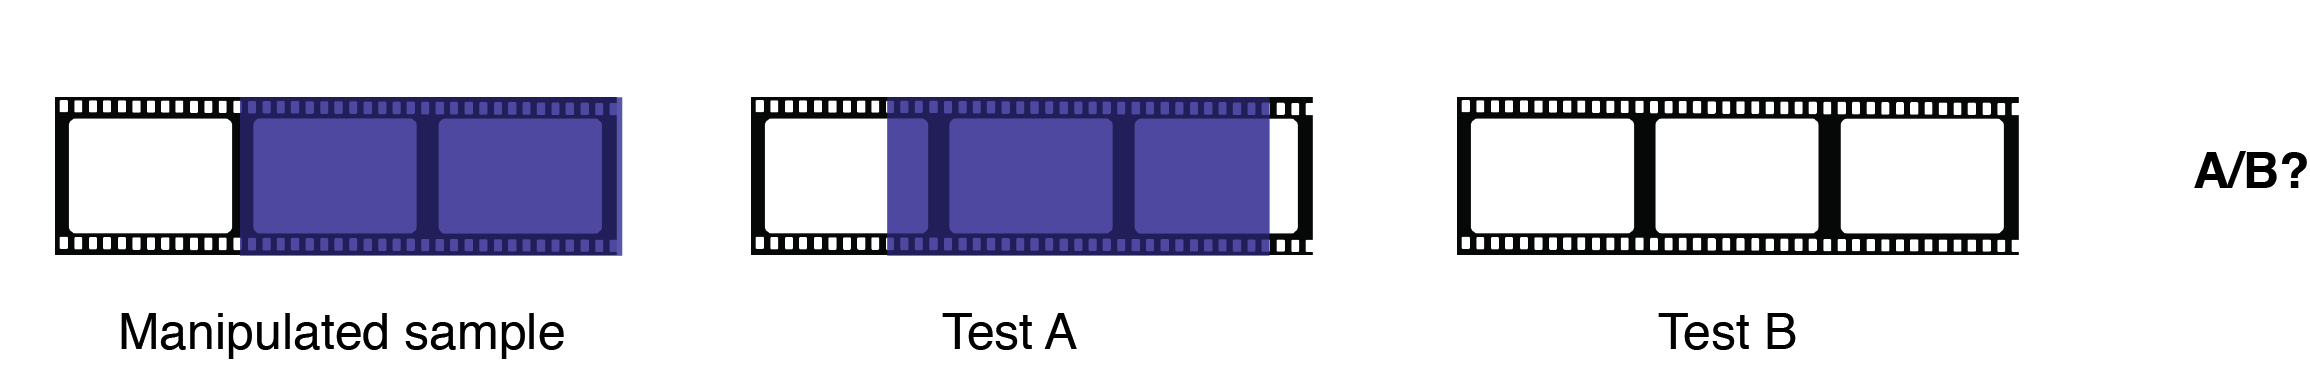
\includegraphics[width=12cm]{img/fire5protocol.png}
                \caption{An altered (filtered or inverted) sample was followed by two untouched tests, one of which contained the sample.}     
        \end{subfigure}
\caption{Experiment 4: design summary and trial structure.}
\end{figure}

\begin{figure}[htp]
\centering
\begin{subfigure}[b]{0.5\textwidth}
\centering
                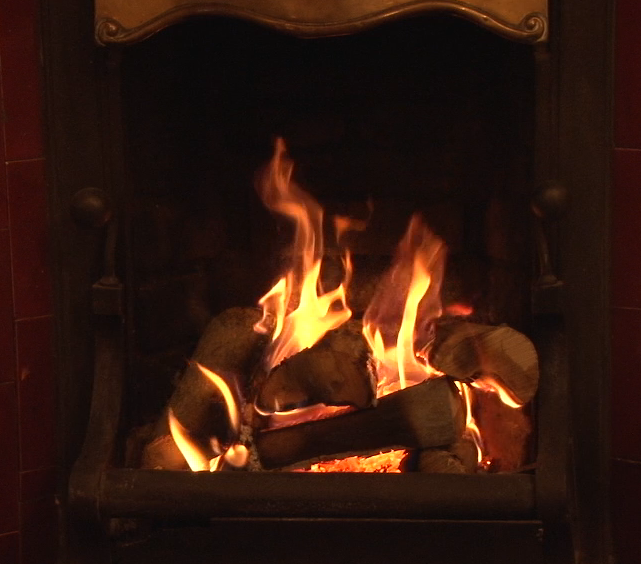
\includegraphics[width=5cm]{img/frame00003.png}
                \caption{Normal}         
        \end{subfigure}\begin{subfigure}[b]{0.5\textwidth}
\centering
                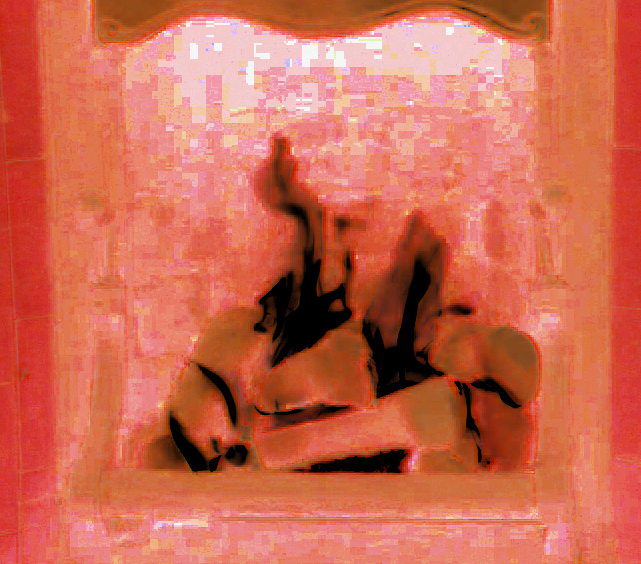
\includegraphics[width=5cm]{img/frame00001.png}
                \caption{Luminance inverted}         
        \end{subfigure}

\begin{subfigure}[b]{0.5\textwidth}
\centering
                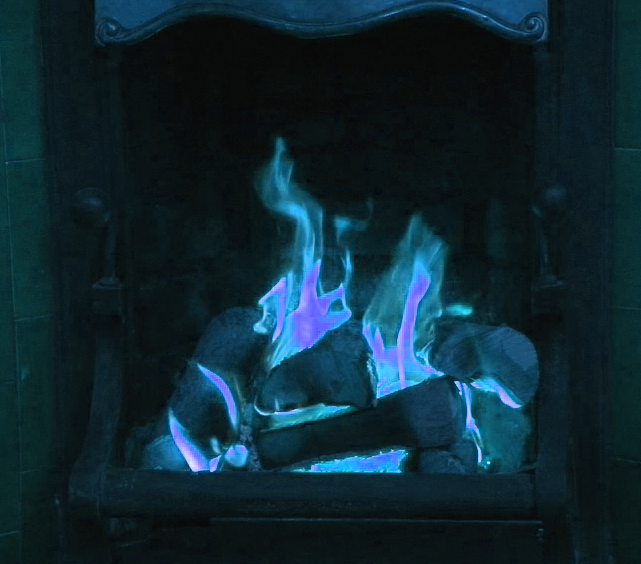
\includegraphics[width=5cm]{img/frame00002.png}
                \caption{Hue inverted}         
        \end{subfigure}\begin{subfigure}[b]{0.5\textwidth}
\centering
                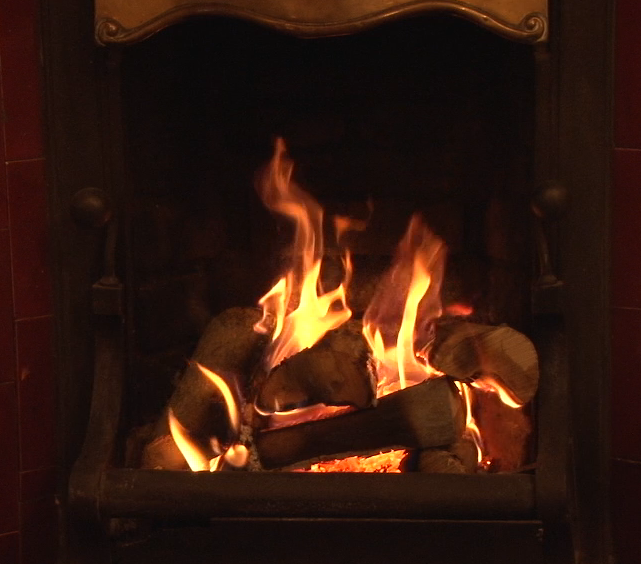
\includegraphics[width=5cm,angle=180]{img/frame00003.png}
                \caption{Spatially inverted}         
        \end{subfigure}

\caption{Experiment 4: Examples of the manipulations we used, applied to one frame. Reversal is not shown.}
\end{figure}

\subsection{Results}

\paragraph{Accuracy by manipulation}

We observed the following mean accuracies:

\begin{center}
\begin{tabular}{ r | l   }
\textbf{Sample manipulation} & \textbf{Mean accuracy}\\
\hline
None&  0.60\\
Negative&  0.59\\
Chromatic& 0.61\\
Reversed&  0.58\\
Inverted&  0.59\\
\end{tabular}
\end{center}

Single-sample $t$-tests showed that subjects were more accurate than chance ($p$<0.05) under each one of these conditions. However, paired-samples $t$-tests showed no difference in means between any pair of conditions ($p$>0.2 in each case).

\paragraph{Learning}

\begin{figure}[htp]
\centering
\begin{subfigure}[b]{\textwidth}
\centering
                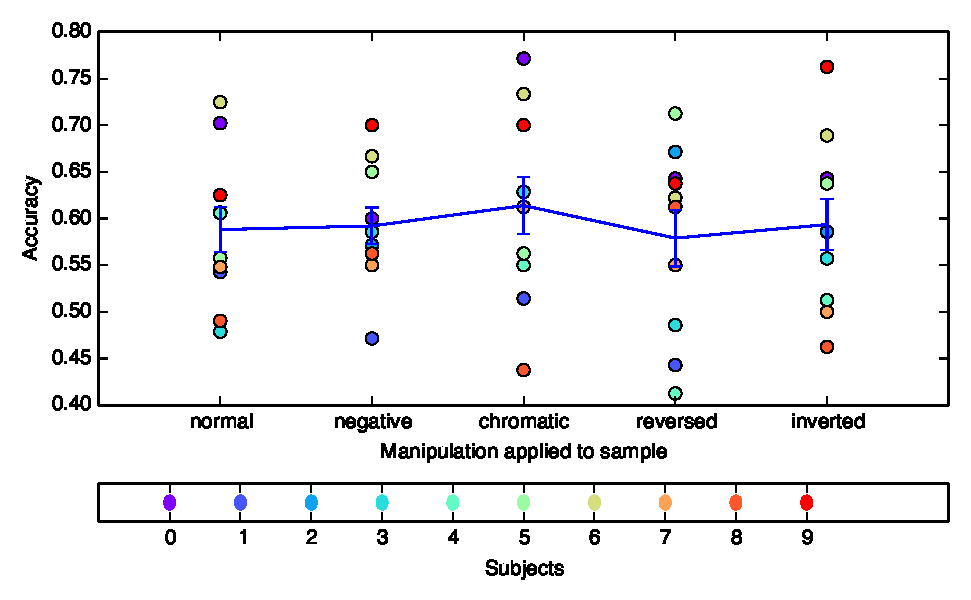
\includegraphics[width=12cm]{img/fig_fire5-manips1_correct_manip.pdf}
                \caption{Accuracy in function of the five manipulations.}
          
        \end{subfigure}

\caption{Experiment 3: Detection was above chance under all manipulations, but was too low to discern a contrast between the effects.}
\end{figure}

\subsection{Discussion}

\section{Experiment 6: colour, inversion and reversal}

\subsection{Methodology}

\paragraph{Stimuli}

A 1000-frame corpus of consecutive fire images was used.



\paragraph{Subjects}

8 subjects were recruited using a mailing list operated by University College London. All reported normal or corrected-to-normal vision.

\paragraph{Trial structure}

Delayed match-to-sample with altered sample.
In each trial, a sample was presented first, followed by two tests. A manipulation was applied to the sample; the tests were unchanged. Subjects indicated which test they thought corresponded to the sample using the left arrow (first sample) and right arrow (second sample) keys. 

Sample length (sL) was one 10 frames (0.2 seconds)
Test length was 15 frames (0.3 seconds)

\paragraph{Factors}

We varied the manipulation applied to the sample clips:
none, colour-inverted, backwards, or spatially inverted.

Colour inversion was done by expressing each image in HSV space and rotating each pixel by 180 degrees about the hue axis.

\paragraph{Block structure}

Firstly, we presented 30 training trials with static samples and tests (displayed for 0.2 and 0.3 seconds respectively) with the four manipulations applied to the sample.

Next, we presented 30 training trials with dynamic samples and tests and the same clip lengths, but with samples and tests unaltered.

We used 4 block types (corresponding to each manipulation) with 4 repetitions of each block (16 blocks total) in random order.


\begin{figure}[H]
\centering
\renewcommand{\arraystretch}{1.8}

      \begin{subfigure}[b]{\textwidth}
\begin{tabular}{ >{\bfseries}r | p{8cm}   }
& \textbf{Experiment 3}\\
\hline
  
Design & 2AFC delayed match-to-sample, with filtered or inverted sample\\                   
Stimuli & 1000-frame corpus\newline
		1 second sample (50 frames)\newline
		1.2 second test (60 frames)\\
Factors & Manipulation:\newline
		a) none\newline
		b) colour inversion\newline
		c) temporal inversion\newline
		d) spatial inversion\\

Block design & Manipulation varied across blocks\newline
		4 block types \newline
		16 blocks in random order \\
Training &60 training trials \\
Subjects&8\\
\end{tabular}
\caption{Design summary.}
   \end{subfigure}

\begin{subfigure}[b]{\textwidth}
\centering
                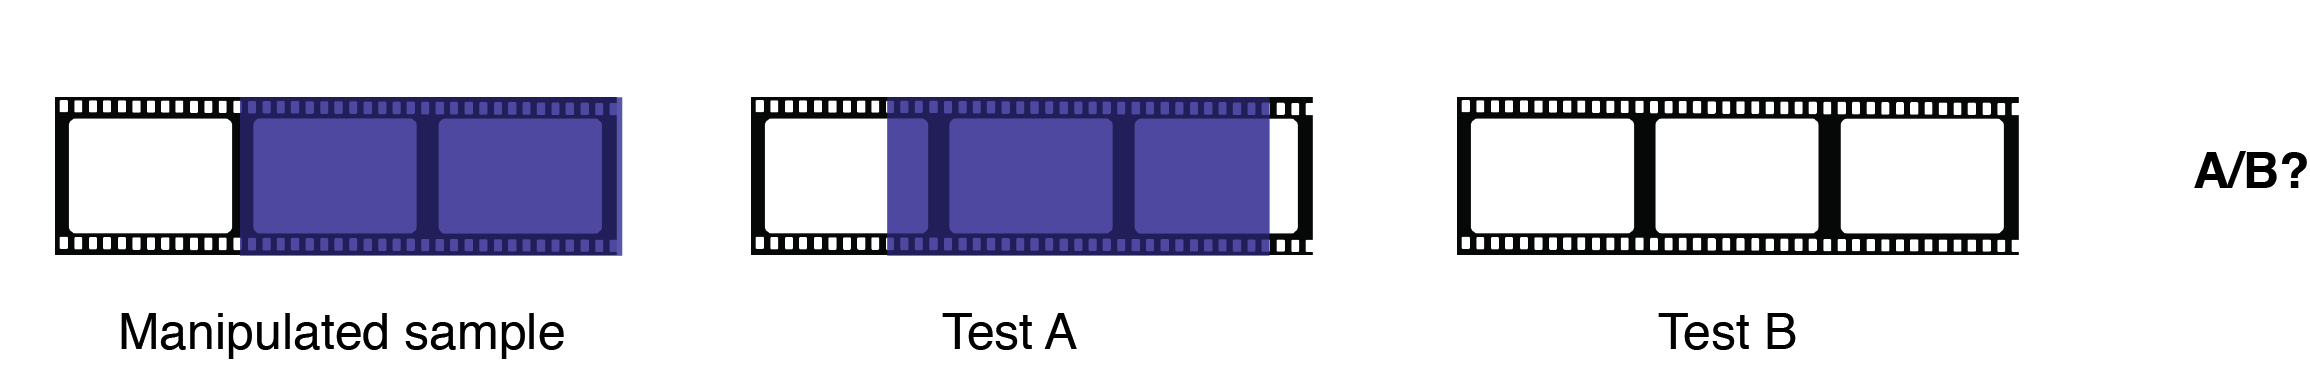
\includegraphics[width=12cm]{img/fire5protocol.png}
                \caption{An altered (filtered or inverted) sample was followed by two untouched tests, one of which contained the sample.}     
        \end{subfigure}
\caption{Experiment 6: design summary and trial structure.}
\end{figure}


\subsection{Results}

\paragraph{Accuracy by manipulation}

The following table shows the mean accuracies for each manipulation, as well as the paired-sample $t$-test $p$-value between that condition and the no-manipulation trials.

\begin{center}
\begin{tabular}{ r | l | l  }
\textbf{Sample manipulation} & \textbf{Mean accuracy} & $p$-value from normal\\
\hline
None&  0.766 & N/A \\
Chromatic& 0.743 & 0.11\\
Reversed&  0.727 & 0.05\\
Inverted&  0.662 & 0.00\\
\end{tabular}
\end{center}

We also note a significant difference between reversion and inversion ($p$=0.03, paired-samples $t$-test). 

All of the conditions gave accuracy greater than chance ($p<$  0.001, single-sample $t$-tests).


\begin{figure}[htp]
\centering

\begin{subfigure}[b]{\textwidth}
\centering
                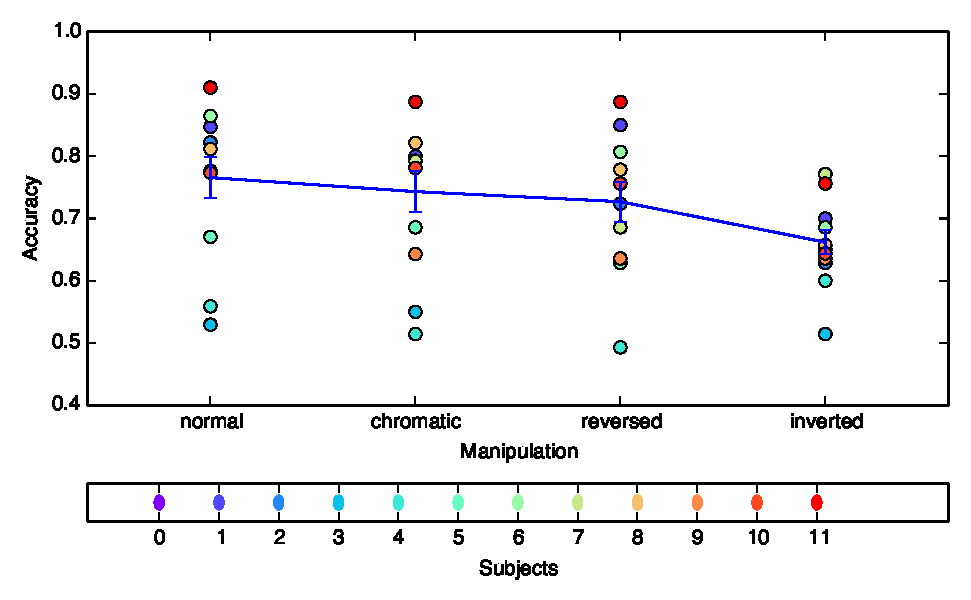
\includegraphics[width=12cm]{img/fig_fire8-manips_correct_manip.pdf}
                \caption{Accuracy against test/sample ratio. Longer tests render the sample harder to find.}
         
        \end{subfigure}
\caption{Experiment 6: effects of each manipulation.}
\end{figure}

\subsection{Discussion}

In terms of design, no-manipulation condition of this experiment exactly replicates the (0.2 second sample, 0.24 second test) condition of experiment 1 (p. \pageref{ex1:accs}). Results were also comparable: accuracy was exactly 0.766 in both cases. As completely different subjects were used, this is useful evidence that we used a large enough sample size.

\paragraph{Colour}
While hue reversal drops the mean by 2 percentage points, a paired-samples $t$-test shows a low probability of difference from the mean ($p$=0.11). Observers do not require the correct colour in order to match fire samples.

\paragraph{Reversal}

Reversing a video clip alters many of its simple motion properties (such as direction of motion) but not certain higher-level motion properties, such as speed. It also does not alter the position of salient motion features: if for example a salient curling flame is tracked in the upper left of the frame, its position will not have changed in the reversed stimulus. Provided that it is just as salient when played in reverse (which small flames usually are, due to their luminance), it will be easily detectable.

Here reversion is associated with a 3.9 percentage point drop in accuracy.

\paragraph{Inversion} 
Inversion alters the local processing of motion features found in fire clips: it transforms upwards motion into downwards motion and leftwards into righwards. It does not, however, alter any of the temporal properties of the clip, either locally or globally.

Inverting a video clip alters the spatial location of all the features contained therein. The signature of a fire clip is not merely a bag of features; each feature is linked to its location in space (``a flare in the the upper left of the frame"). This information is disrupted by inversion.

Here inversion is associated with a 10 percentage point drop in accuracy.

\paragraph{Comparison}

The accuracy drop under inversion (10 p.p.) is much larger than that under reversal (3.9 p.p). For clips of length 0.2 s, then, spatial properties are much more important than temporal properties. Subjects are helped much more by knowing where features are in the image, than when they occur.

Subjects definitely have \textit{some} temporal resolution during the 0.2 second period: persistence of vision blurs details together within a window of 0.04 s\cite{edridge1945persistence}, a much shorter duration than the clips shown here. However, the information derived from the spatial location of features is much more important than temporal information.


\chapter{Temporal search for faces}

\section{Face stimuli}

We also used several different portrait video clips of facial motion, recorded at 50fps. We show the frame counts here:

50fps

x3\_Free	2538
xs\_HCB		830
x3\_TGDoY	1064
x3\_TTLs	1332
x4\_Free	2208
x4\_HCB		814
x4\_TGODoY	1002
x4\_TTLS	1158
x5\_Free	1830
x5\_HCB		798
x5\_TGODoY	859
x5\_TTLS	1318
x8\_Free	2937
x8\_HCB		737
x8\_TGODoY	958
x8\_TTLS	1306

These clips consisted of either free facial motion (the subject was instructed to speak freely) or video of the subject singing along with nursery rhymes.

\section{Experiment n: visual search for faces with short tests}

\subsection{Methodology}

\subsection{Results}

\subsection{Discussion}

\chapter{Temporal search for faces and fire}


\section{Experiment n: Loading the perceptual system with faces and fire}

\subsection{Methodology}

\paragraph{Stimuli}

A 10,000-frame corpus of consecutive fire images was used.



\paragraph{Subjects}

8 subjects were recruited using a mailing list operated by University College London. All reported normal or corrected-to-normal vision.

\paragraph{Trial structure}

Yes-no dual delayed match-to-sample.
In each trial, we presented two tests (one fire clip and one face clip), followed by two samples(one fire clip and one face clip). After each test, subjects indicated whether they thought it matched the corresponding test (up arrow) or not (down arrow).

We thus derived two accuracy measures: fire accuracy and face accuracy.

Sample lengths were all 100 frames (2 s) and test lengths were all 120 frames (2.4 s).

\paragraph{Factors}

We varied the order in which samples were shown (fire first or face first).
We always showed the fire test before the face test.

\paragraph{Block structure}

No training trials were used.



\chapter{Modelling}

\section{Forgetting functions}



\chapter{Discussion}


\section{Hierarchies}




Are the top-down/bottom-up continuum and the automatic/deliberate continuum actually the same thing?

\chapter{Unsorted}

\section{Characterising fire}

\section {Evolutionary value}

From an evolutionary point of view, mastery of fire was key to human development. Being able to control fire allowed early humans to cook food, defend themselves from predators and survive in cold, challenging environments. Fire was the first of a long line of technologies which release stored energy from fuel and turn it to human purposes; the earliest archaeological evidence of fire use dates back 1.8 million years, with frequent use found from 100,000 years ago\cite{bowman2009fire}. Even before this, hominids regularly encountered flame in the form of bushfires, although these were perceived as a threat, not a controllable, exploitable entity.

The evolving human visual system has therefore been exposed to a large amount of flamelike stimuli in the last 1.8 million years. These stimuli have often appeared in dangerous or life-threatening contexts, either posing a threat or aiding survival. In sufficiently extreme situations, such as extreme cold or heavy predation, those early humans who could successfully control fire had an increased chance of survival.

It is therefore natural to enquire whether the human visual system has become adapted in any way to the perception of flamelike stimuli. Does the visual system employ any specific representations or specialised models when attending to fire, does it use the same general-purpose systems employed when observing a novel moving stimulus?

This question recalls the ongoing debate concerning the specialisation of face perception. We find increased activation of the fusiform face area and inferior temporal sulcus while viewing faces\cite{allison2000social}; this can be explained either by innate specialisation or learned proficiency. In the same way, observation of fire may recruit neurons and systems which respond preferentially to, and perform better on, flame stimuli. On the other hand, observing fire may stimulate the same neural populations as observing other moving stimuli.

\section{High-level and low-level representations}

The goal of neuroscience is to impose structure and explanatory power on the neural systems present in the brain. This task is accomplished using descriptions in several different domains of representation:



\begin{figure}[htp]
\renewcommand{\arraystretch}{1.8}
\begin{tabular}{ >{\bfseries}r | p{8cm}   }
& \textbf{Experiment 1}\\
\hline
  
	Design & 2AFC delayed match-to-sample (sample clip followed by two test clips)\\                   
  Stimuli & 1000-frame corpus \\
  Factors & sample length (10, 25, 50) frames or (0.2, 0.5, 1)seconds. \newline 
sample/test ratio (1.2 1.4 1.6 1.8 2).\\
  Block design & Sample length varied across blocks\newline
			Test length varied within blocks \newline
			15 conditions \newline
40 trials per condition \newline
600 trials \newline
25 training trials \\
\end{tabular}
\end{figure}

\begin{table}[htdp]
\caption{default}
\begin{center}
\begin{tabular}{|c|c|}

\end{tabular}
\end{center}
\label{default}
\end{table}%



\begin{singlespace}
\begin{footnotesize}
\begin{twocolumn}
\bibliographystyle{unsrt}
\bibliography{references,bib_litreview}
\end{twocolumn}
\end{footnotesize}
\end{singlespace}
\newpage

Appendices here

\end{document}



